\section{Wyniki badań i ich omówienie}\label{Wyniki badań i ich omówienie}

\subsection{Charakterystyka badanej grupy} % cbg

% Należy przedstawić:
%   + liczbę respondentów,
%   + płeć,
%   + wiek,
%   + kierunek studiów,
%   + rok studiów,
%   + aktywność fizyczną.

\begin{table}[h!]
    \centering
    \caption{Płęć badanych}
    \label{tab:plec-badanych}
    \begin{tabular}{|l|l|l|}
        \hline
        Płeć & n & \% \\
        \hline
        \hline
        Kobieta & 90 & 84.1 \\
        \hline
        Mężczyzna & 17 &  15.9\\
        \hline
    \end{tabular}
\end{table}

\begin{table}[h!]
    \centering
    \caption{Wiek badanych}
    \label{tab:wiek}
    \begin{tabular}{|l|l|l|}
        \hline
        Wiek & n & \% \\
        \hline
        \hline
        < 20 & 10 & 9.3 \\
        \hline
        20–22 & 14 & 13.1 \\
        \hline
        23–25 & 24 & 22.4 \\
        \hline
        >25 & 59 & 55.1 \\
        \hline
    \end{tabular}
\end{table}

\begin{table}[h!]
    \centering
    \caption{Rok studiów}
    \label{tab:rok-studiow}
    \begin{tabular}{|l|l|l|}
        \hline
        Rok studiów	& n & \% \\
        \hline
        \hline
        I & 11 & 10.3 \\
        \hline
        II & 11 & 10.3 \\
        \hline
        III & 15 & 14 \\
        \hline
        IV & 40 & 37.4 \\
        \hline
        V & 12 & 11.2 \\
        \hline
        Studia magisterskie uzupełniające & 18 & 16.8 \\
        \hline
    \end{tabular}
\end{table}

\begin{table}[h!]
    \centering
    \caption{Kierunki studiów}
    \label{tab:kierunki-studiow}
    \begin{tabular}{|l|l|l|}
        \hline
        Kierunek studiów & n & \% \\
        \hline
        \hline
        Psychologia & 51 & 47.2 \\
        \hline
        Dietetyka & 27 & 25 \\
        \hline
        Informatyka & 4 & 3.7 \\
        \hline
        Filologia & 3 & 2.7 \\
        \hline
        Finanse i rachunkowość & 3 & 2.7 \\
        \hline
        Fizjoterapia & 3 & 2.7 \\
        \hline
        Logistyka & 3 & 2.7 \\
        \hline
        Business & 2 & 1.8\\
        \hline
        Kryminologia i kryminalistyka & 2 & 1.8 \\
        \hline
        Medycyna & 2 & 1.8 \\
        \hline
        Prawo & 2 & 1.8 \\
        \hline
        Psychologia i psychoterapia & 2 & 1.8 \\
        \hline
        Administracja & 1 & 0.9 \\
        \hline
        Behawiorystyka i psychologia zwierząt & 1 & 0.9 \\
        \hline
        Bezpieczeństwo wewnętrzne & 1 & 0.9 \\
        \hline
        Mediacja sztuki & 1 & 0.9 \\
        \hline
    \end{tabular}
\end{table}

\begin{table}[h!]
    \centering
    \caption{Aktywność fizyczna}
    \label{tab:aktywnosc fizyczna}
    \begin{tabular}{|l|l|l|}
        \hline
        Aktywność fizyczna & n & \% \\
        \hline
        \hline
        Nigdy & 4 & 3.7 \\
        \hline
        Rzadziej niż raz w tygodniu & 36 & 33.6 \\
        \hline
        1–2 razy w tygodniu	& 28 & 26.2 \\
        \hline
        3–4 razy w tygodniu & 25 & 23.4 \\
        \hline
        5 lub więcej razy w tygodniu & 14 & 13.1 \\
        \hline
    \end{tabular}
\end{table}

%%%%%%%%%%%%%%%%%%%%%%%%%%%%%%

\begin{figure}
    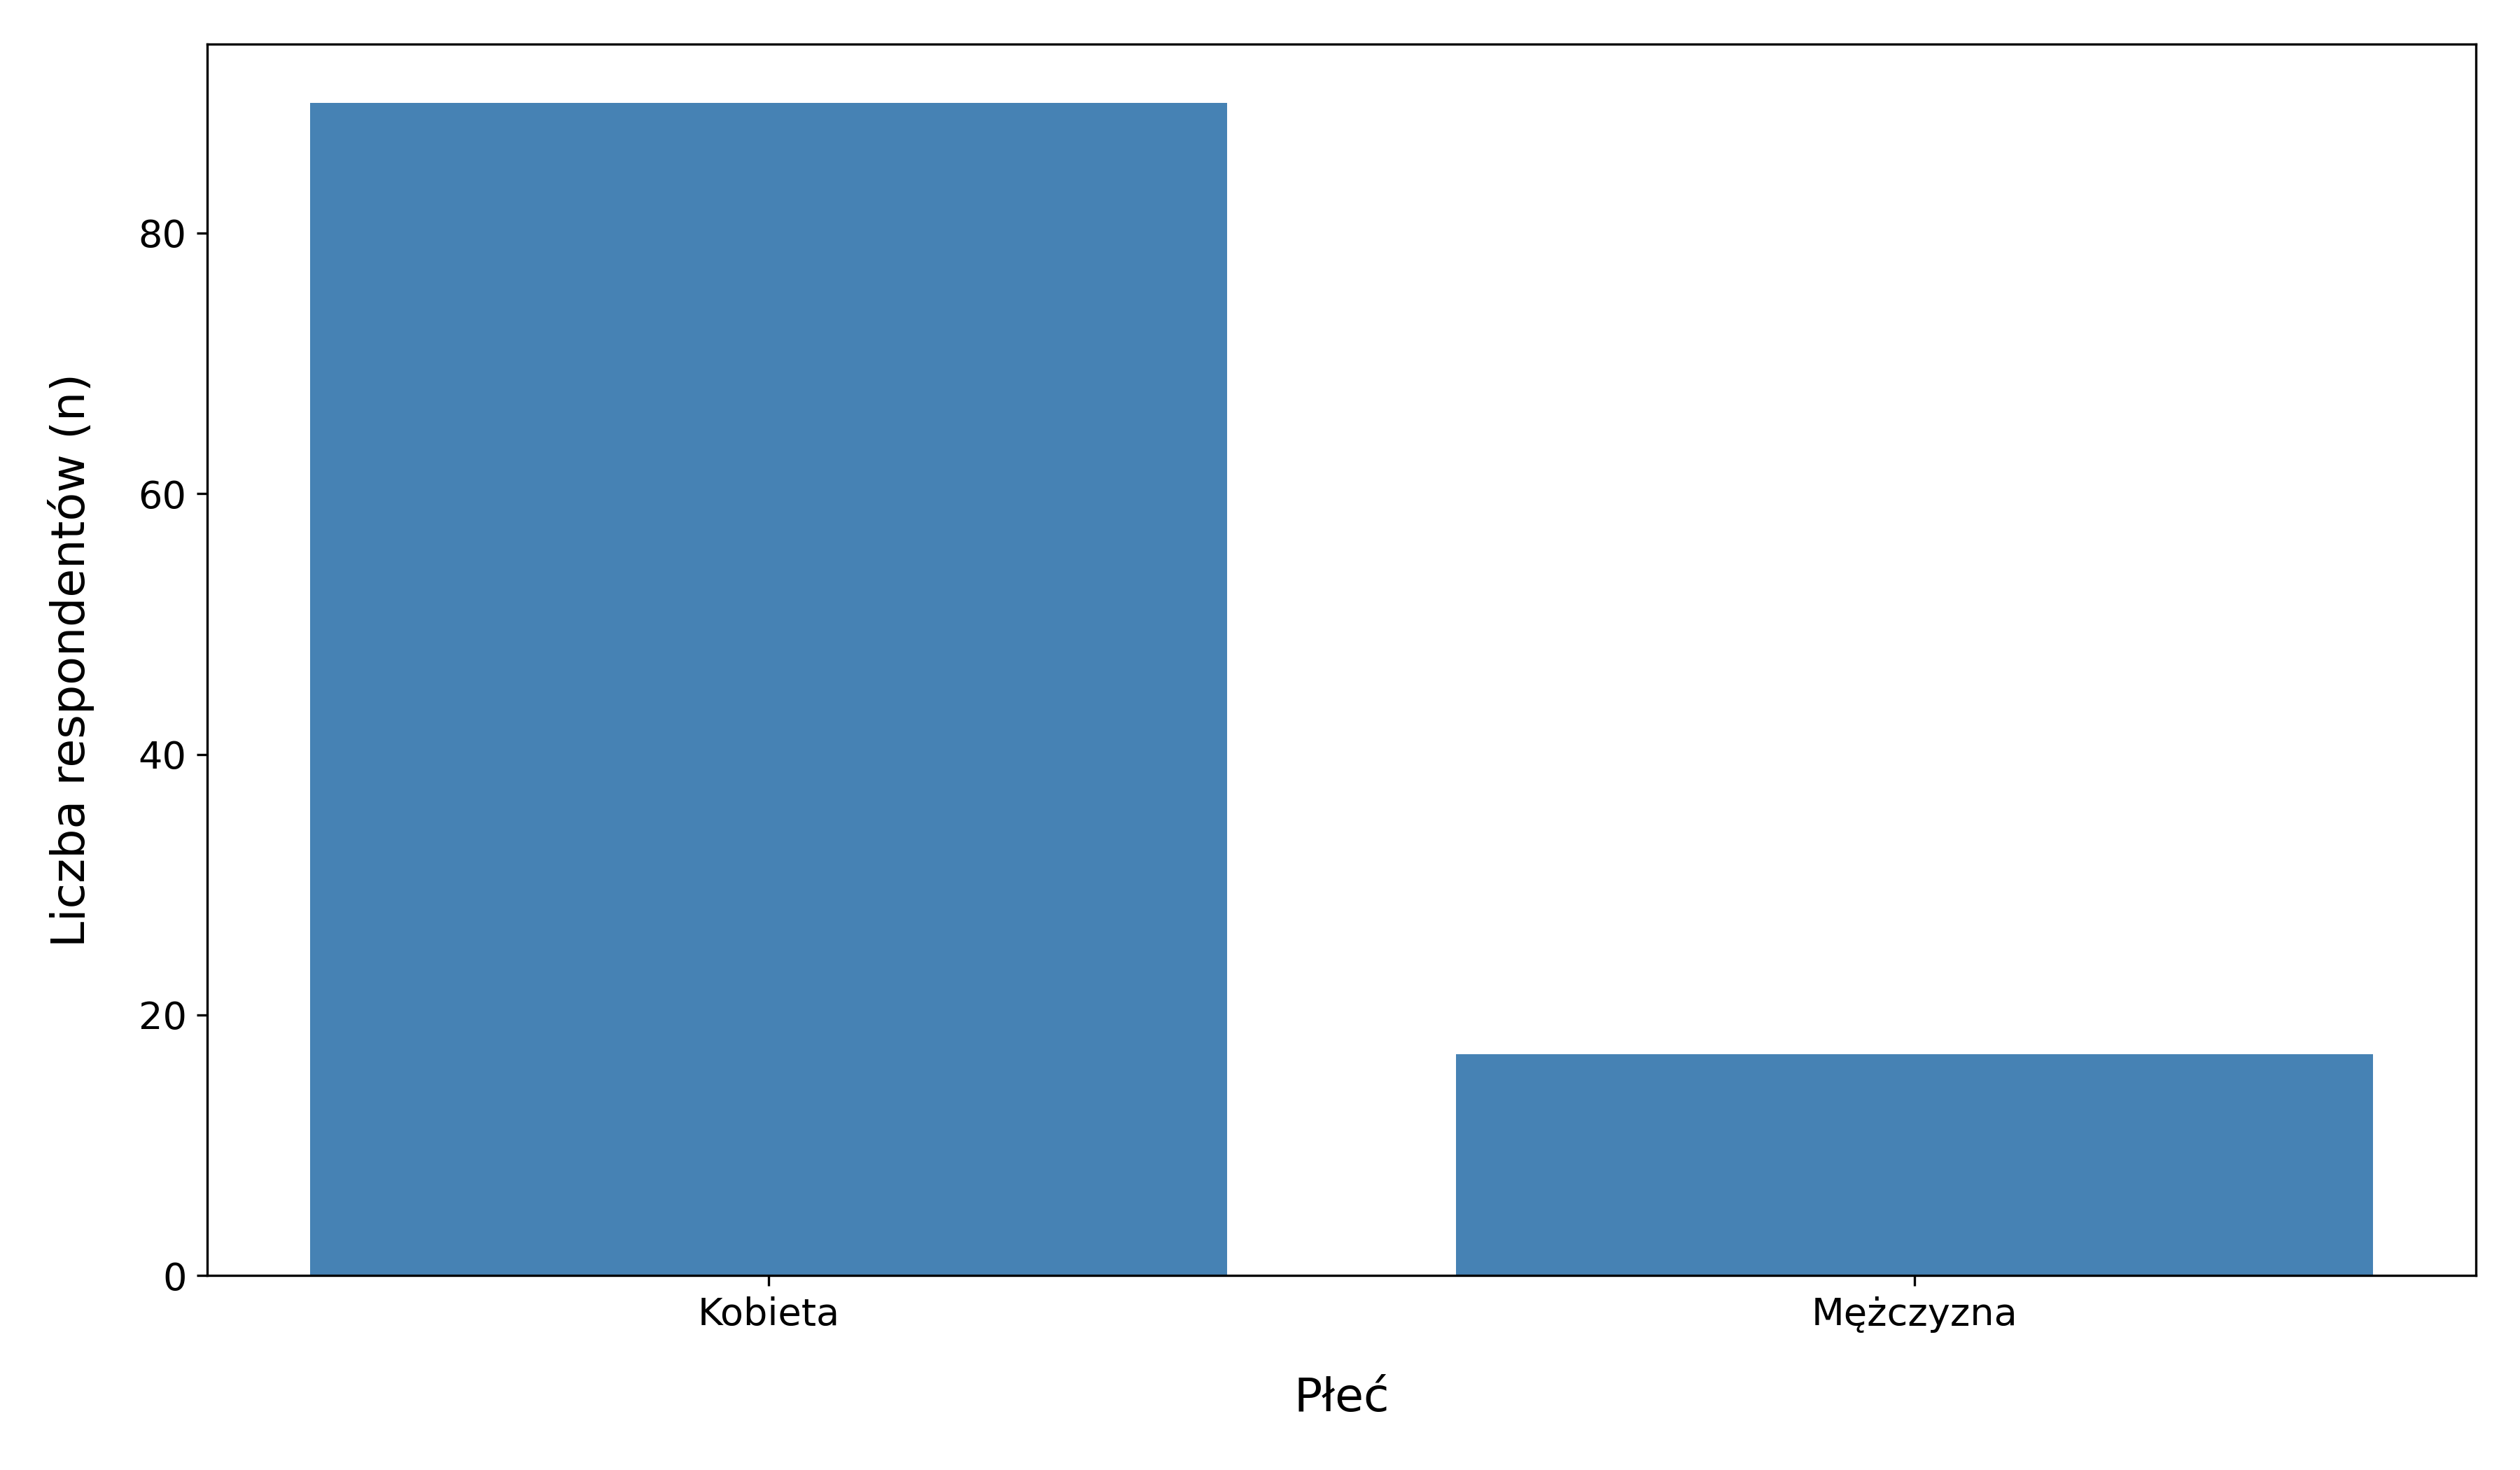
\includegraphics[width=\textwidth]{plots/plec-badanych.png}
    \centering
    \caption{Wykres słupkowy pokazujący liczbę respondentów poszczególnych płci.}
    \label{fig:plec}
\end{figure}

\begin{figure}
    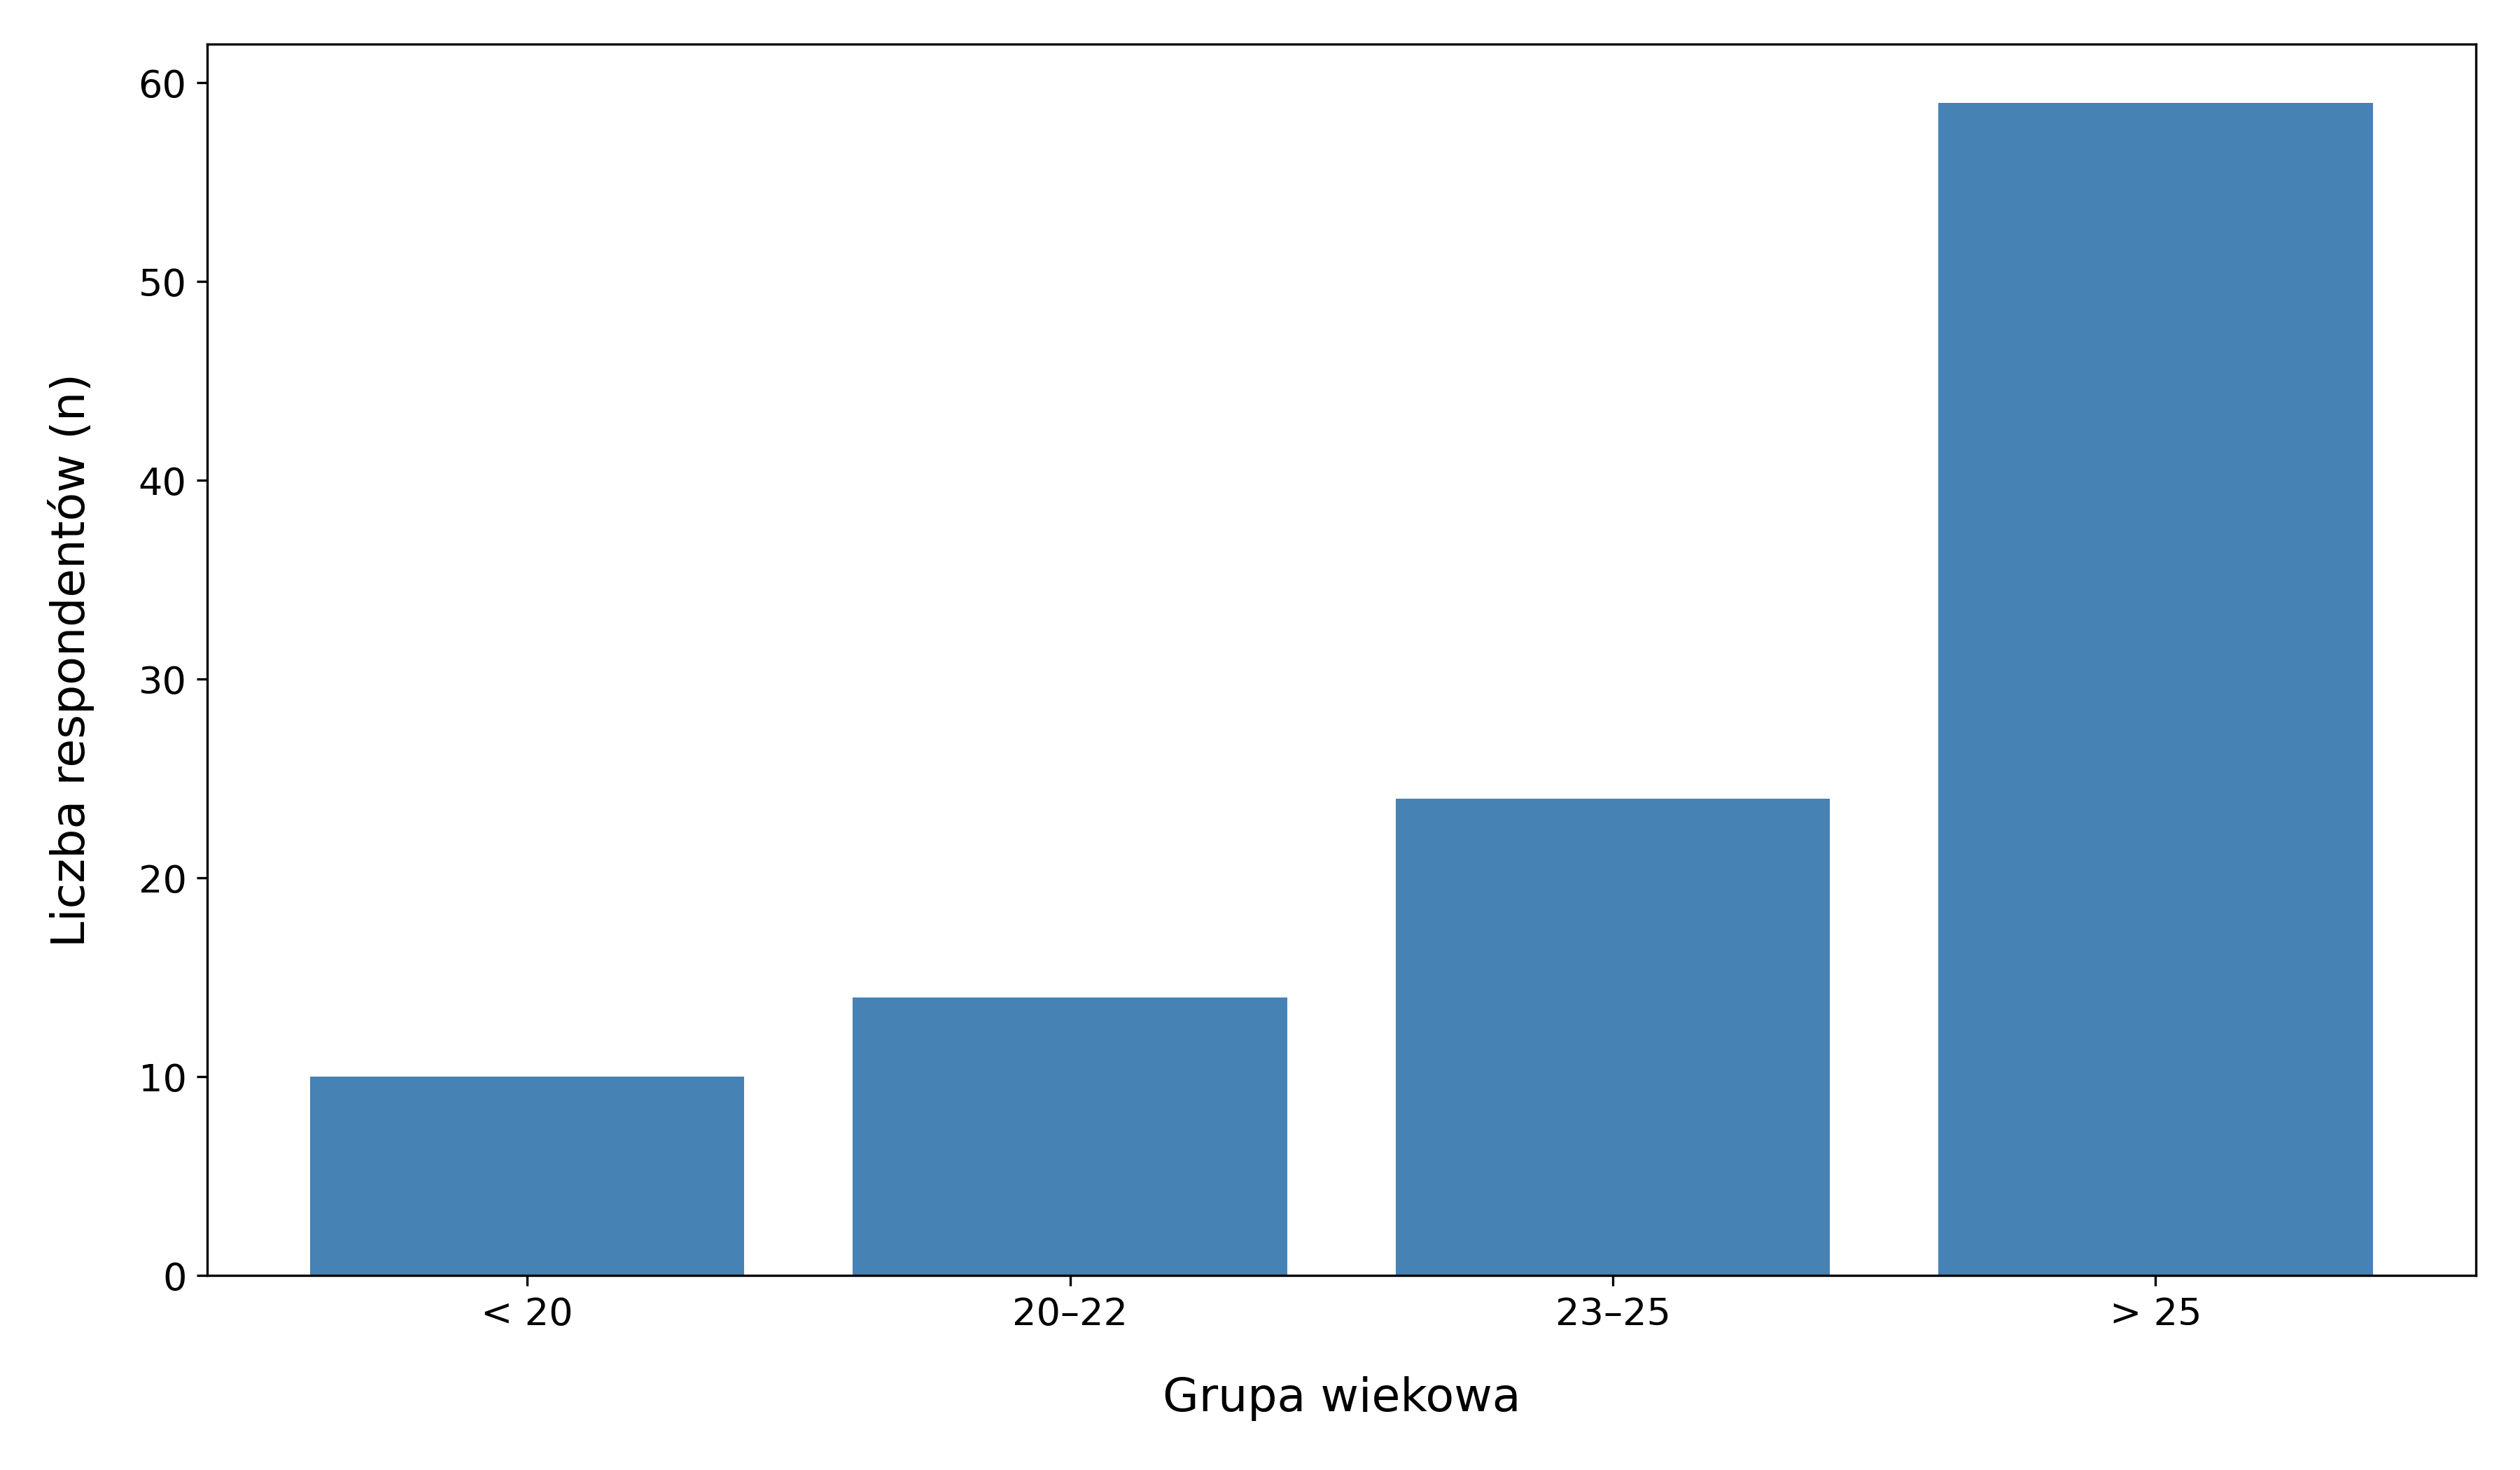
\includegraphics[width=\textwidth]{plots/wiek-badanych.png}
    \centering
    \caption{Wykres słupkowy pokazujący liczbę respondentów w poszczególnych grupach wiekowych.}
    \label{fig:wiek}
\end{figure}

\begin{figure}
    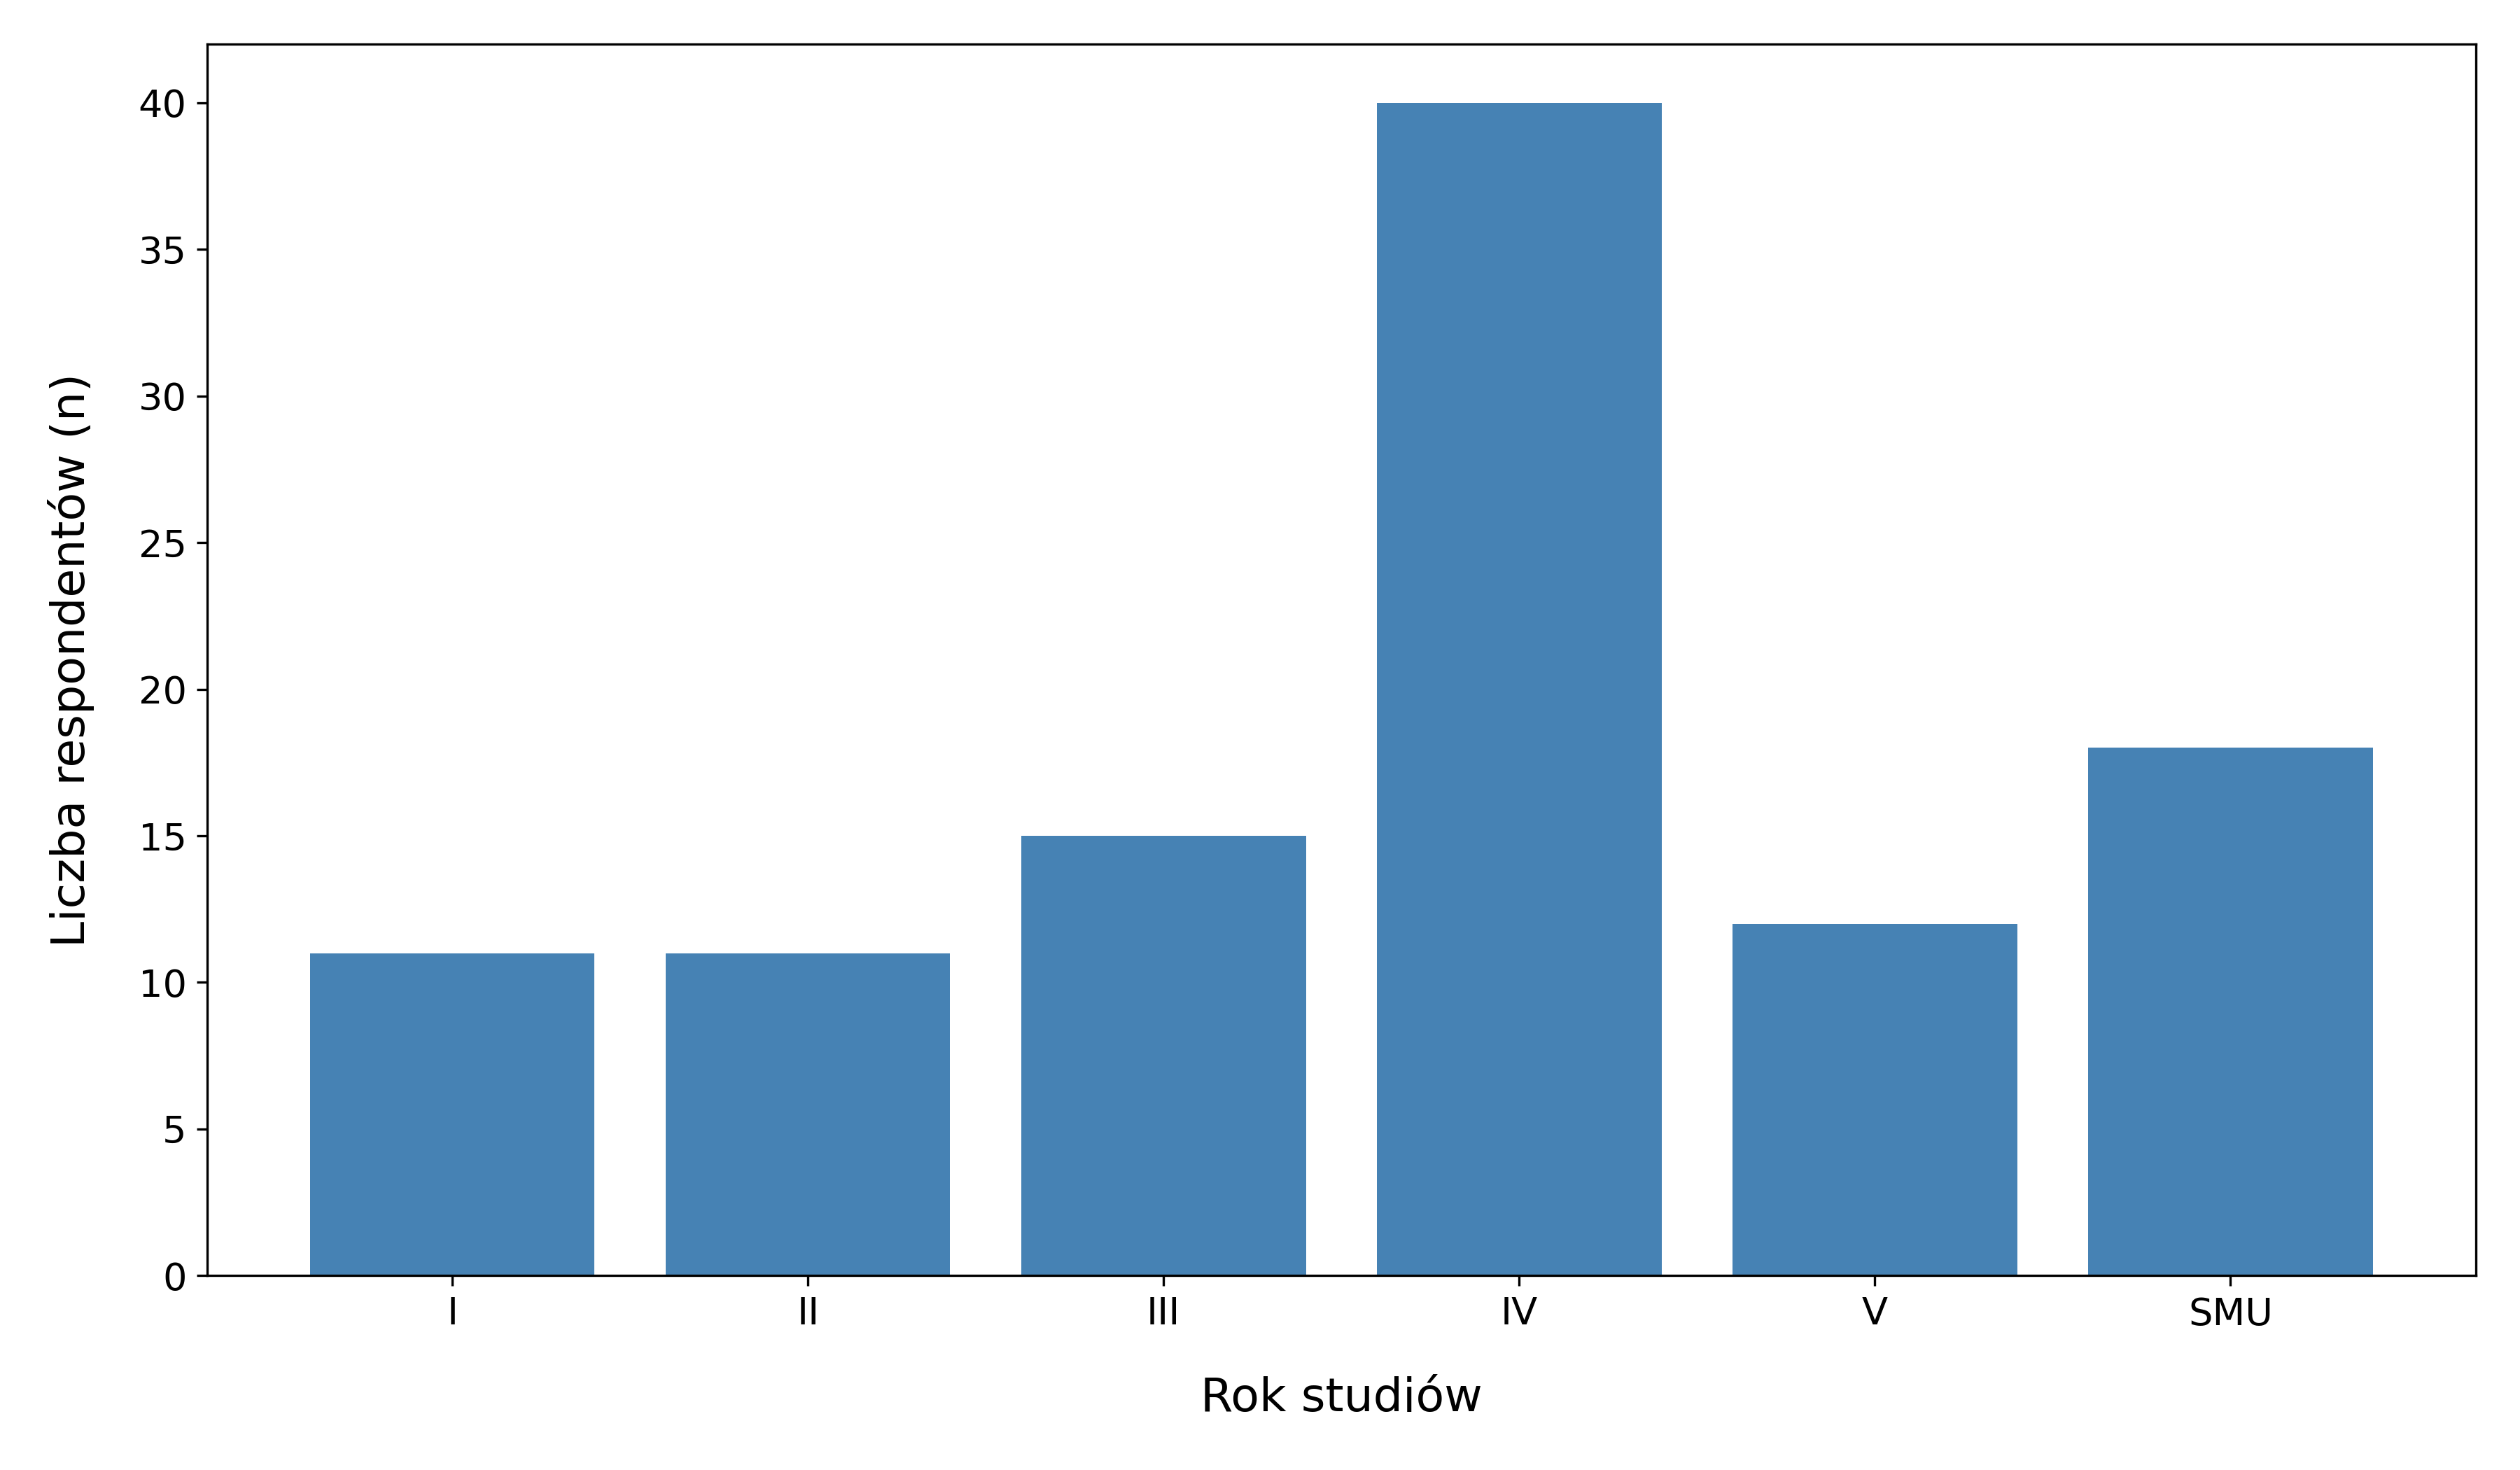
\includegraphics[width=\textwidth]{plots/rok-studiow.png}
    \centering
    \caption{Wykres słupkowy pokazujący liczbę respondentów na poszczególnych latach studiów. Zastosowane skróty: SMU - Studia magisterskie uzupełniające.}
    \label{fig:rok-studiow}
\end{figure}

\begin{figure}
    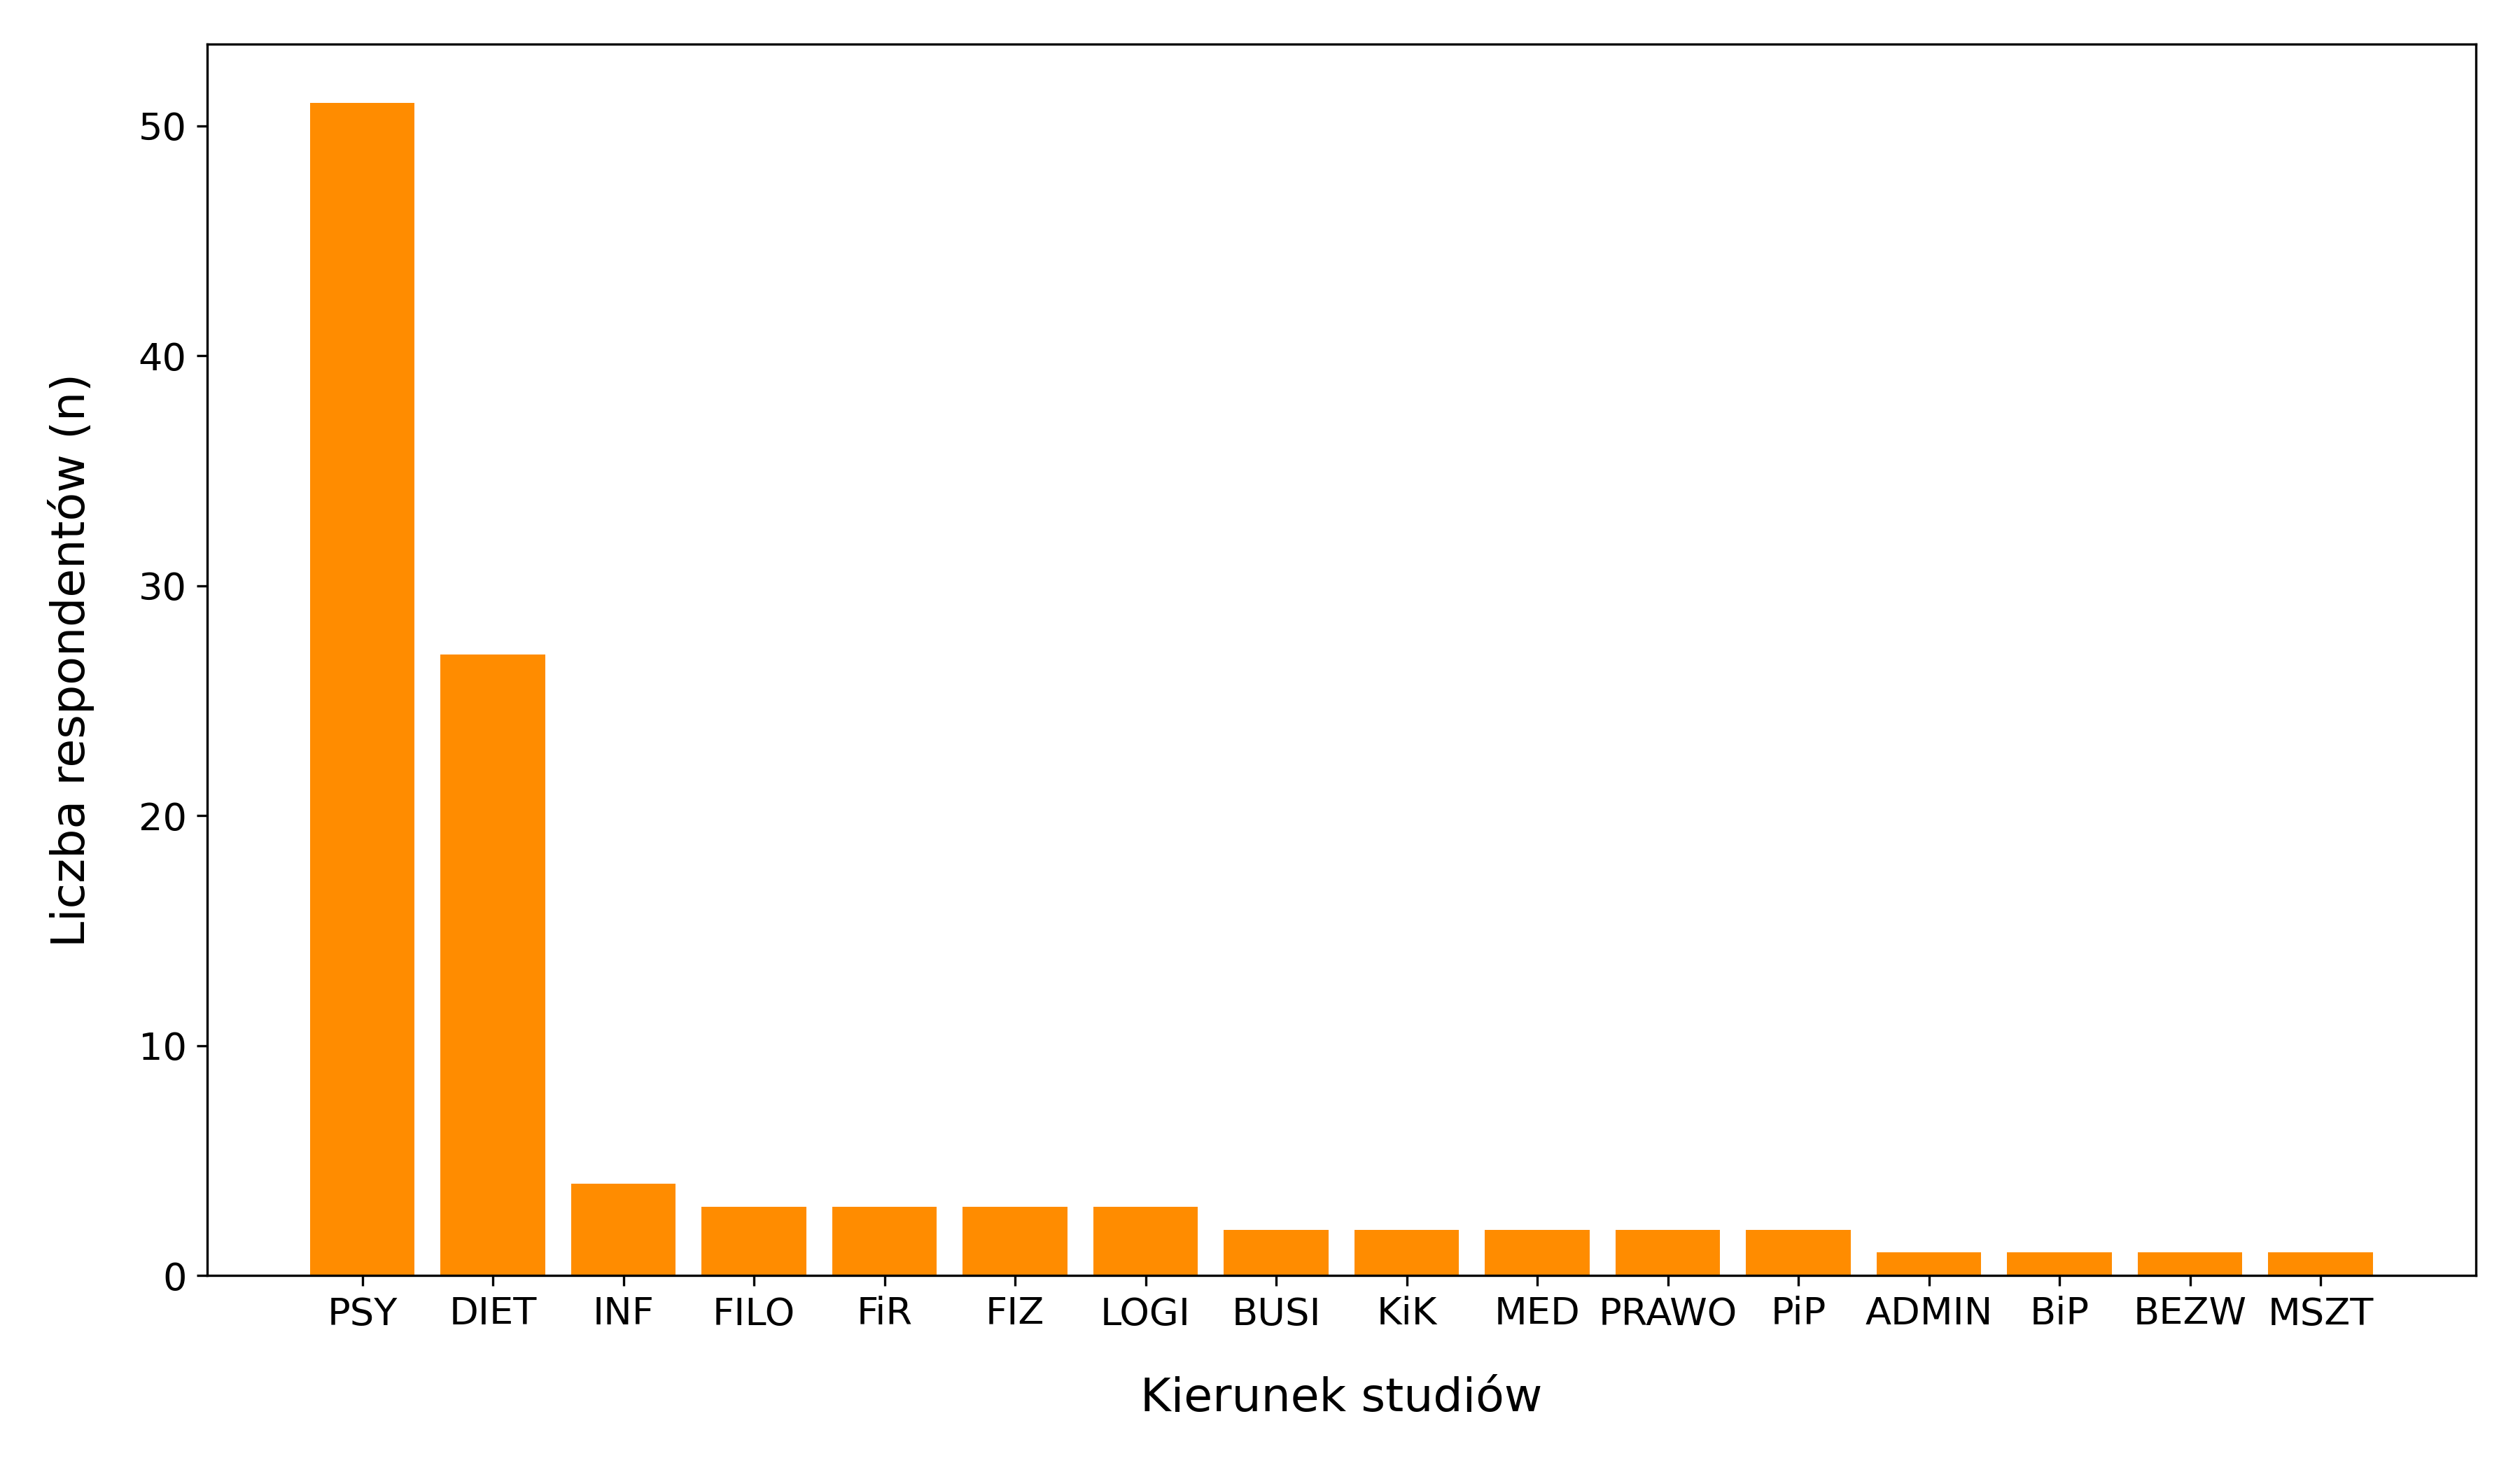
\includegraphics[width=\textwidth]{plots/kierunki-studiow.png}
    \centering
    \caption{Wykres słupkowy pokazujący liczbę respondentów ze względu na ich kierunek studiów. Zastosowane skróty: PSY - Psychologia, DIET - Dietetyka, INF - Informatyka, FILO - Filologia, FiR - Finanse i rachunkowość, FIZ - Fizjoterapia, LOGI - Logistyka, BUSI - Business, KiK - Kryminologia i kryminalistyka, MED - Medycyna, PRAWO - Prawo, PiP - Psychologia i psychoterapia, ADMIN - Administracja, BiP - Behawiorystyka i psychologia zwierząt, BEZW - Bezpieczeństwo wewnętrzne, MSZT - Mediacja sztuki).}
    \label{fig:kierunki-studiow}
\end{figure}

\begin{figure}
    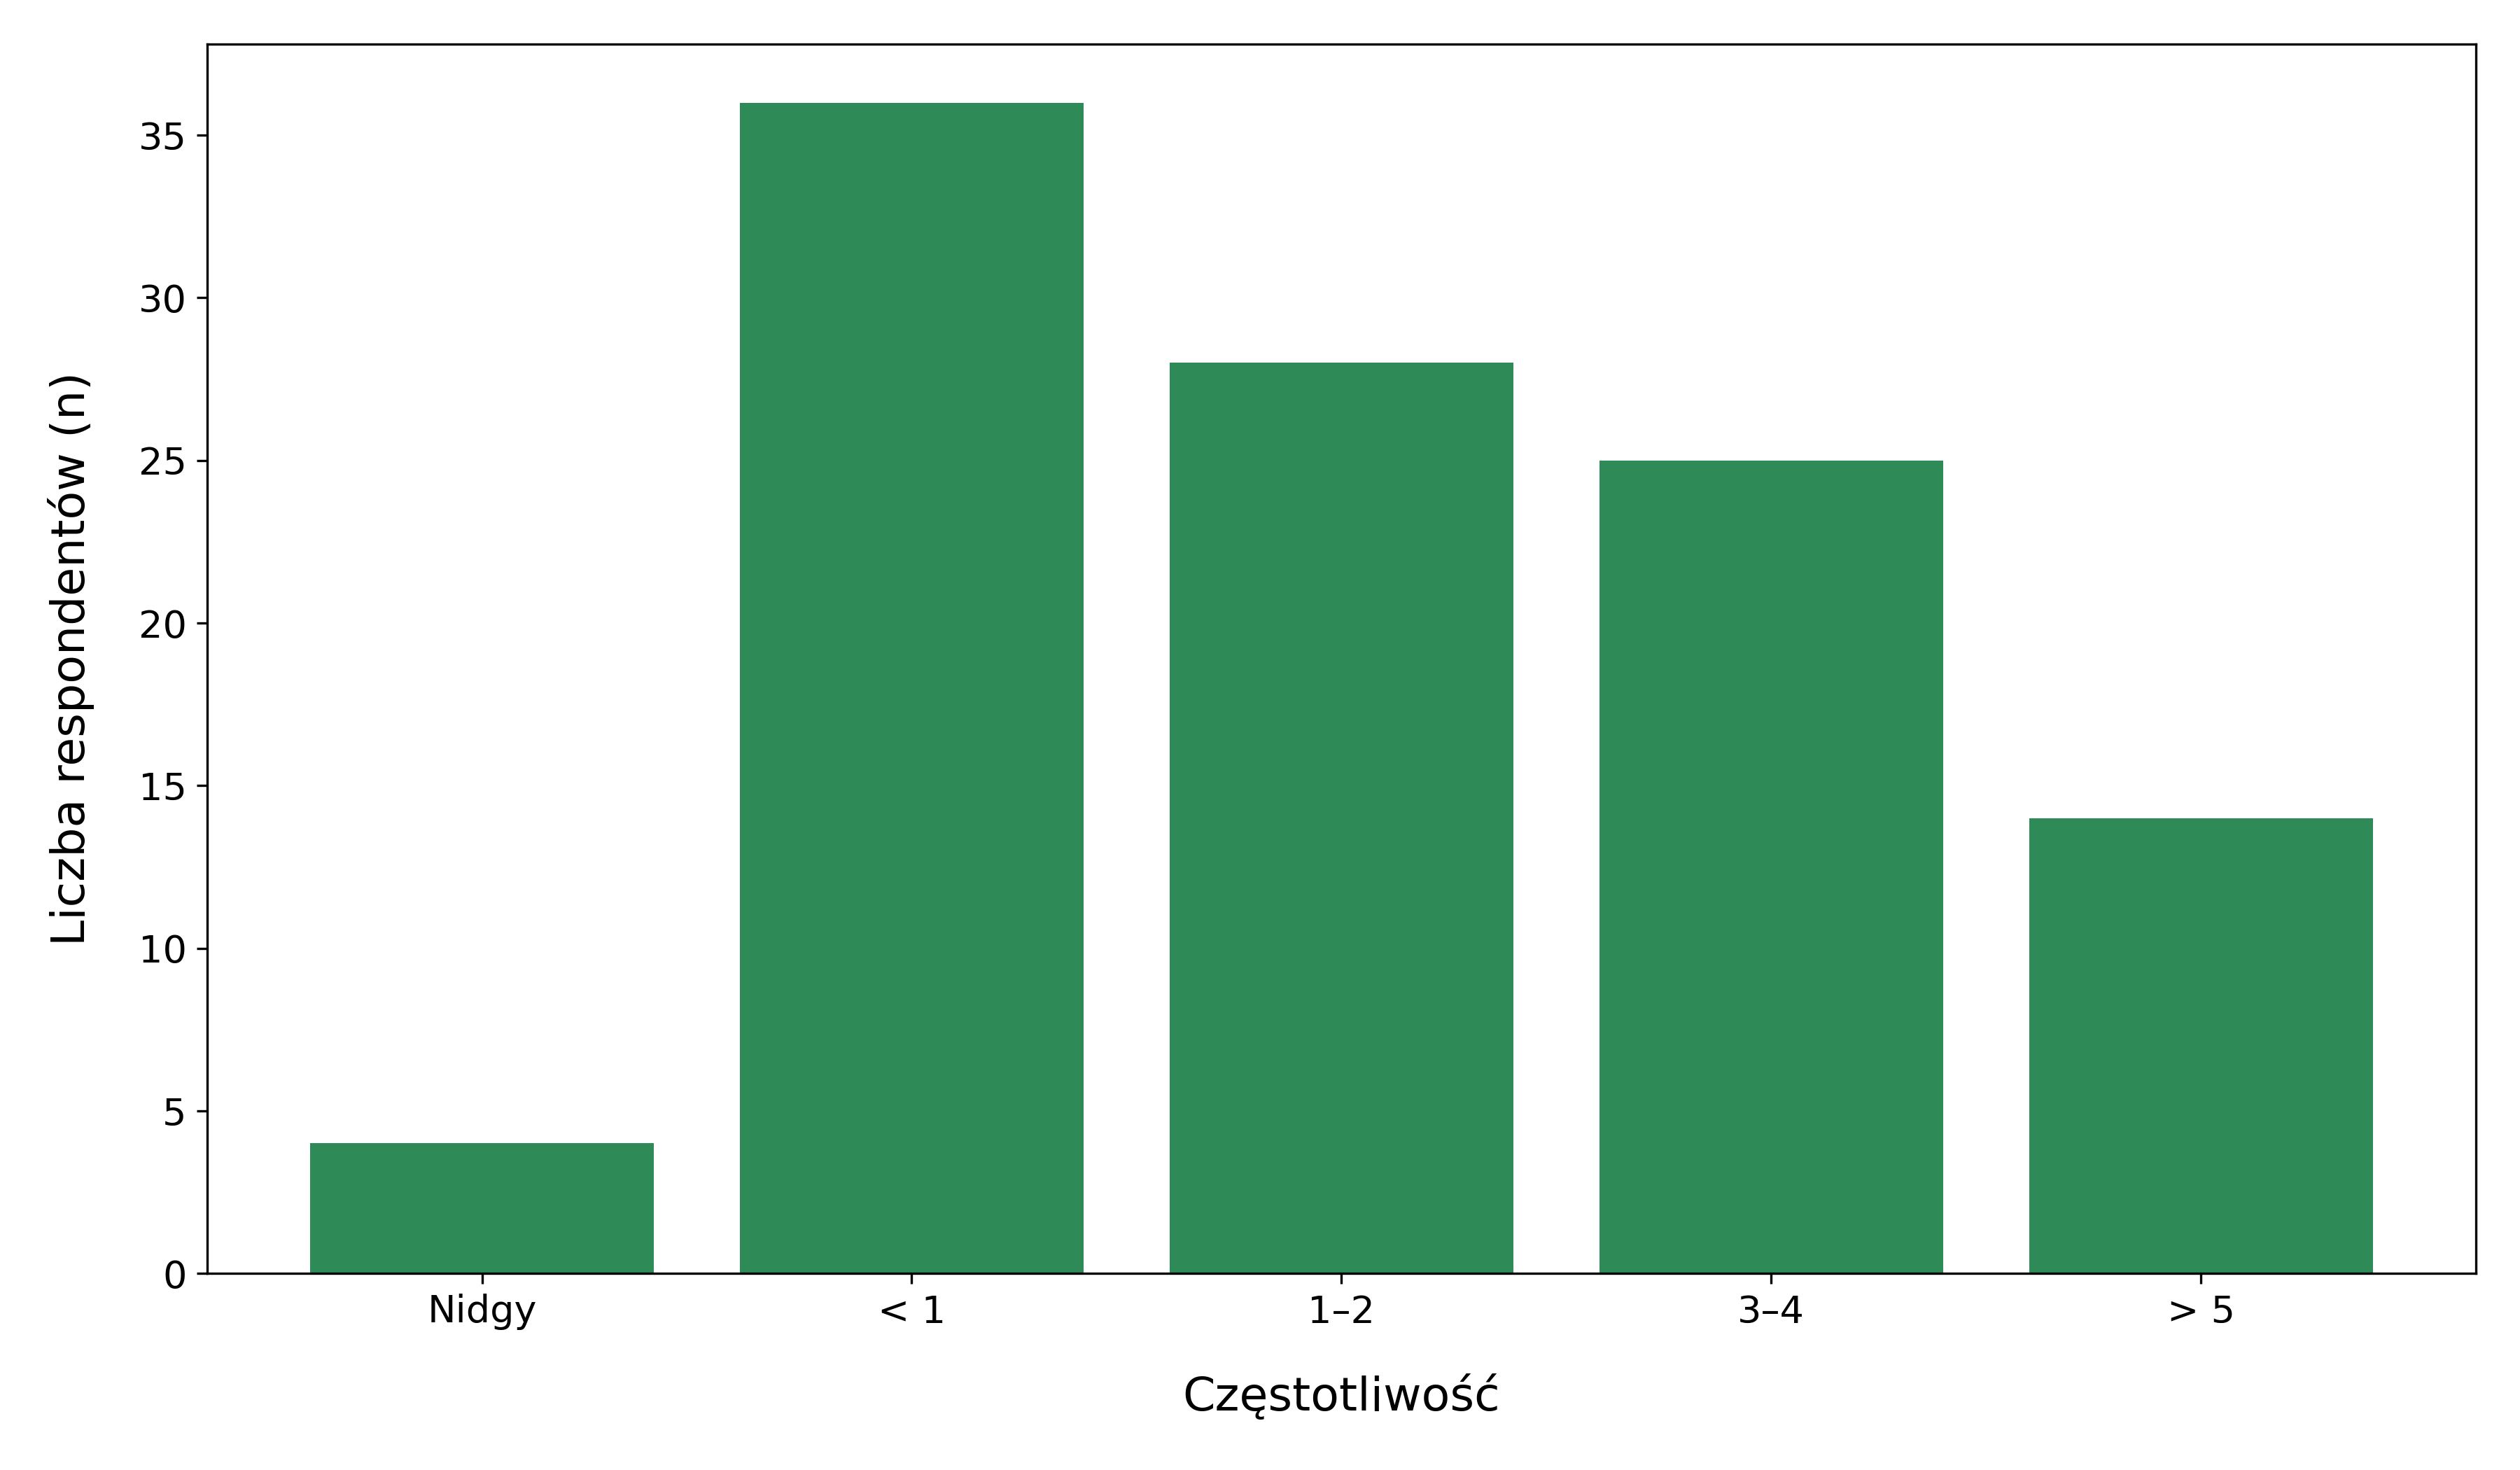
\includegraphics[width=\textwidth]{plots/aktywnosc-fizyczna.png}
    \centering
    \caption{Wykres słupkowy pokazujący częstość wykonywania aktywności fizycznej wśród respondentów.}
    \label{fig:aktywnosc-fizyczna}
\end{figure}


\subsection{Częstość stosowania suplementów}

% Należy przedstawić, ilu studentów aktualnie stosuje suplementy diety.

% Czy aktualnie stosujesz suplementy?, n, %

\begin{table}[h!]
    \centering
    \caption{Aktualne stosowanie suplementów}
    \label{tab:akt-stos-supl}
    \begin{tabular}{|l|l|l|}
        \hline
        Aktualne stosowanie suplementów & n & \% \\
        \hline
        \hline
        Tak & 97 & 90.7 \\
        \hline
        Nie & 10 & 9.3 \\
        \hline
    \end{tabular}
\end{table}

\begin{figure}
    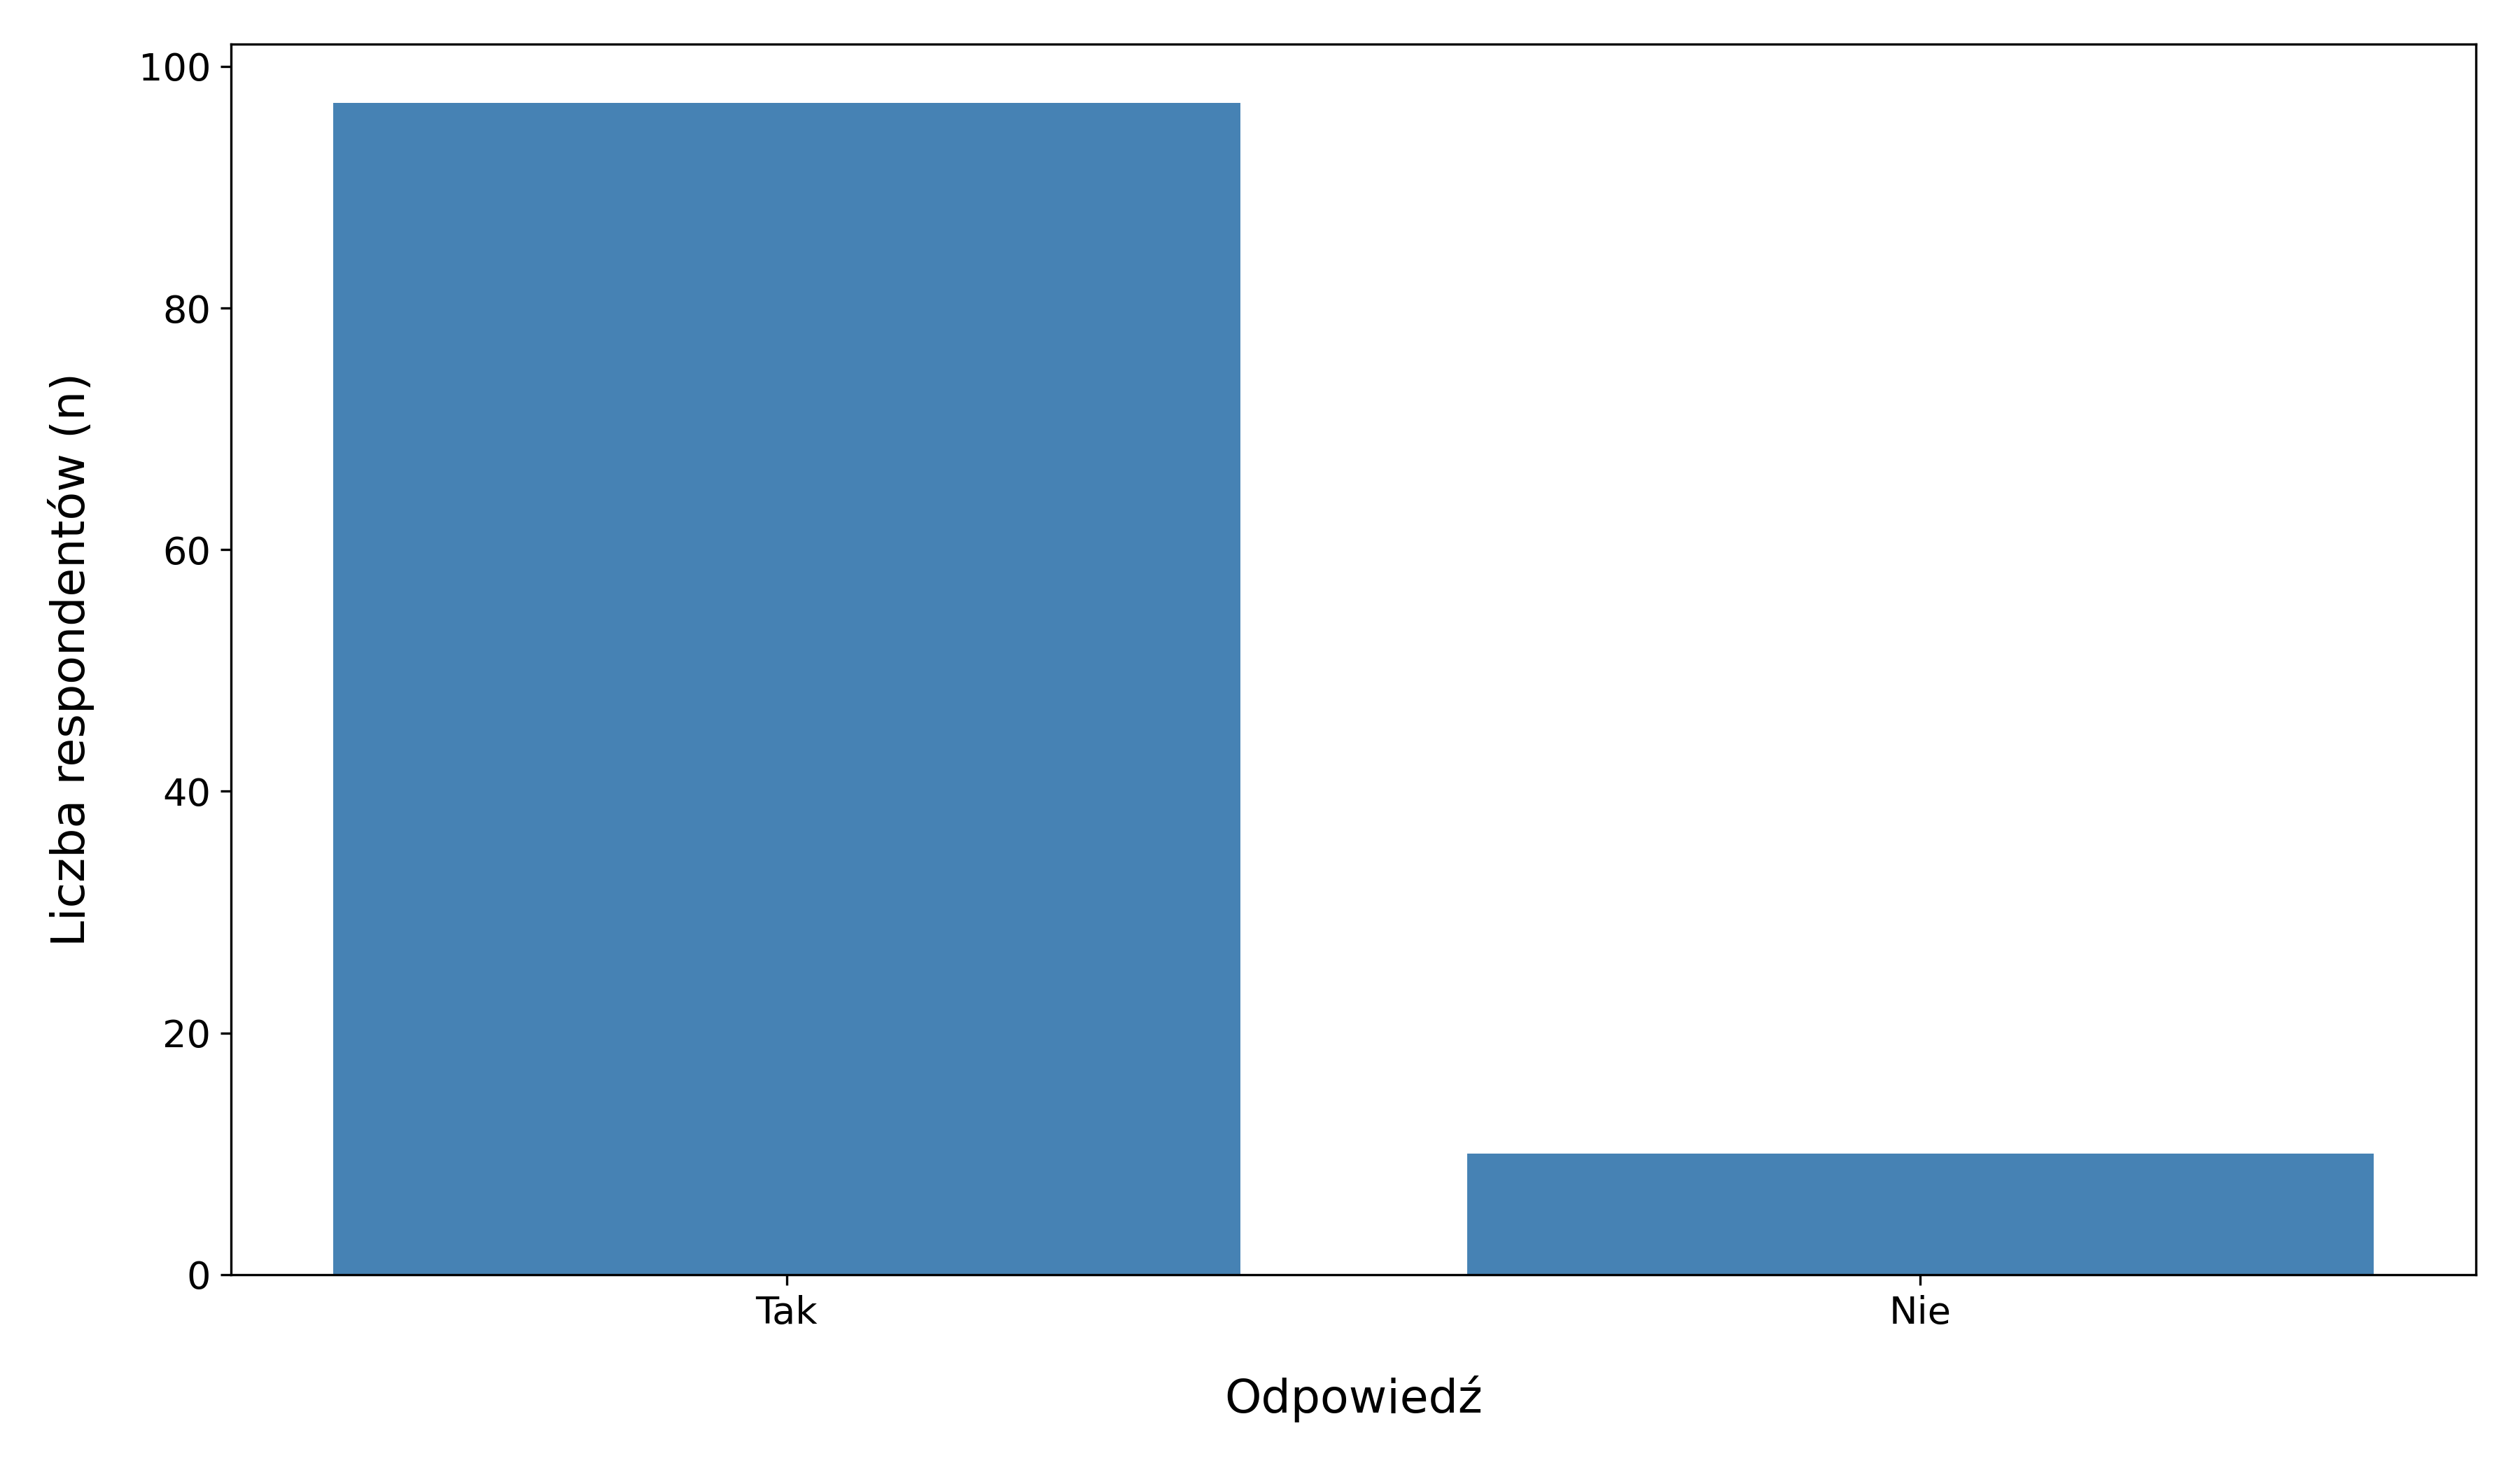
\includegraphics[width=\textwidth]{plots/aktualne-suplementy.png}
    \centering
    \caption{Wykres słupkowy pokazujący aktualne stosowanie suplementów w grupie badawczej.}
    \label{fig:akt-stos-supl}
\end{figure}

% NOTE
% Adjust all below based on whether participant take suplements

% Częstość stosowania suplementów

\begin{table}[h!]
    \centering
    \caption{Częstość stosowanie suplementów}
    \label{tab:cze-stos-supl}
    \begin{tabular}{|l|l|l|}
        \hline
        Częstość stosowania & n & \% \\
        \hline
        \hline
        Codziennie & 63 & 64.95 \\
        \hline
        Kilka razy w tygodniu & 21 & 21.65 \\
        \hline
        Kilka razy w miesiącu & 3 & 3.1 \\
        \hline
        Sporadycznie & 10 & 10.3 \\
        \hline
    \end{tabular}
\end{table}

\begin{figure}
    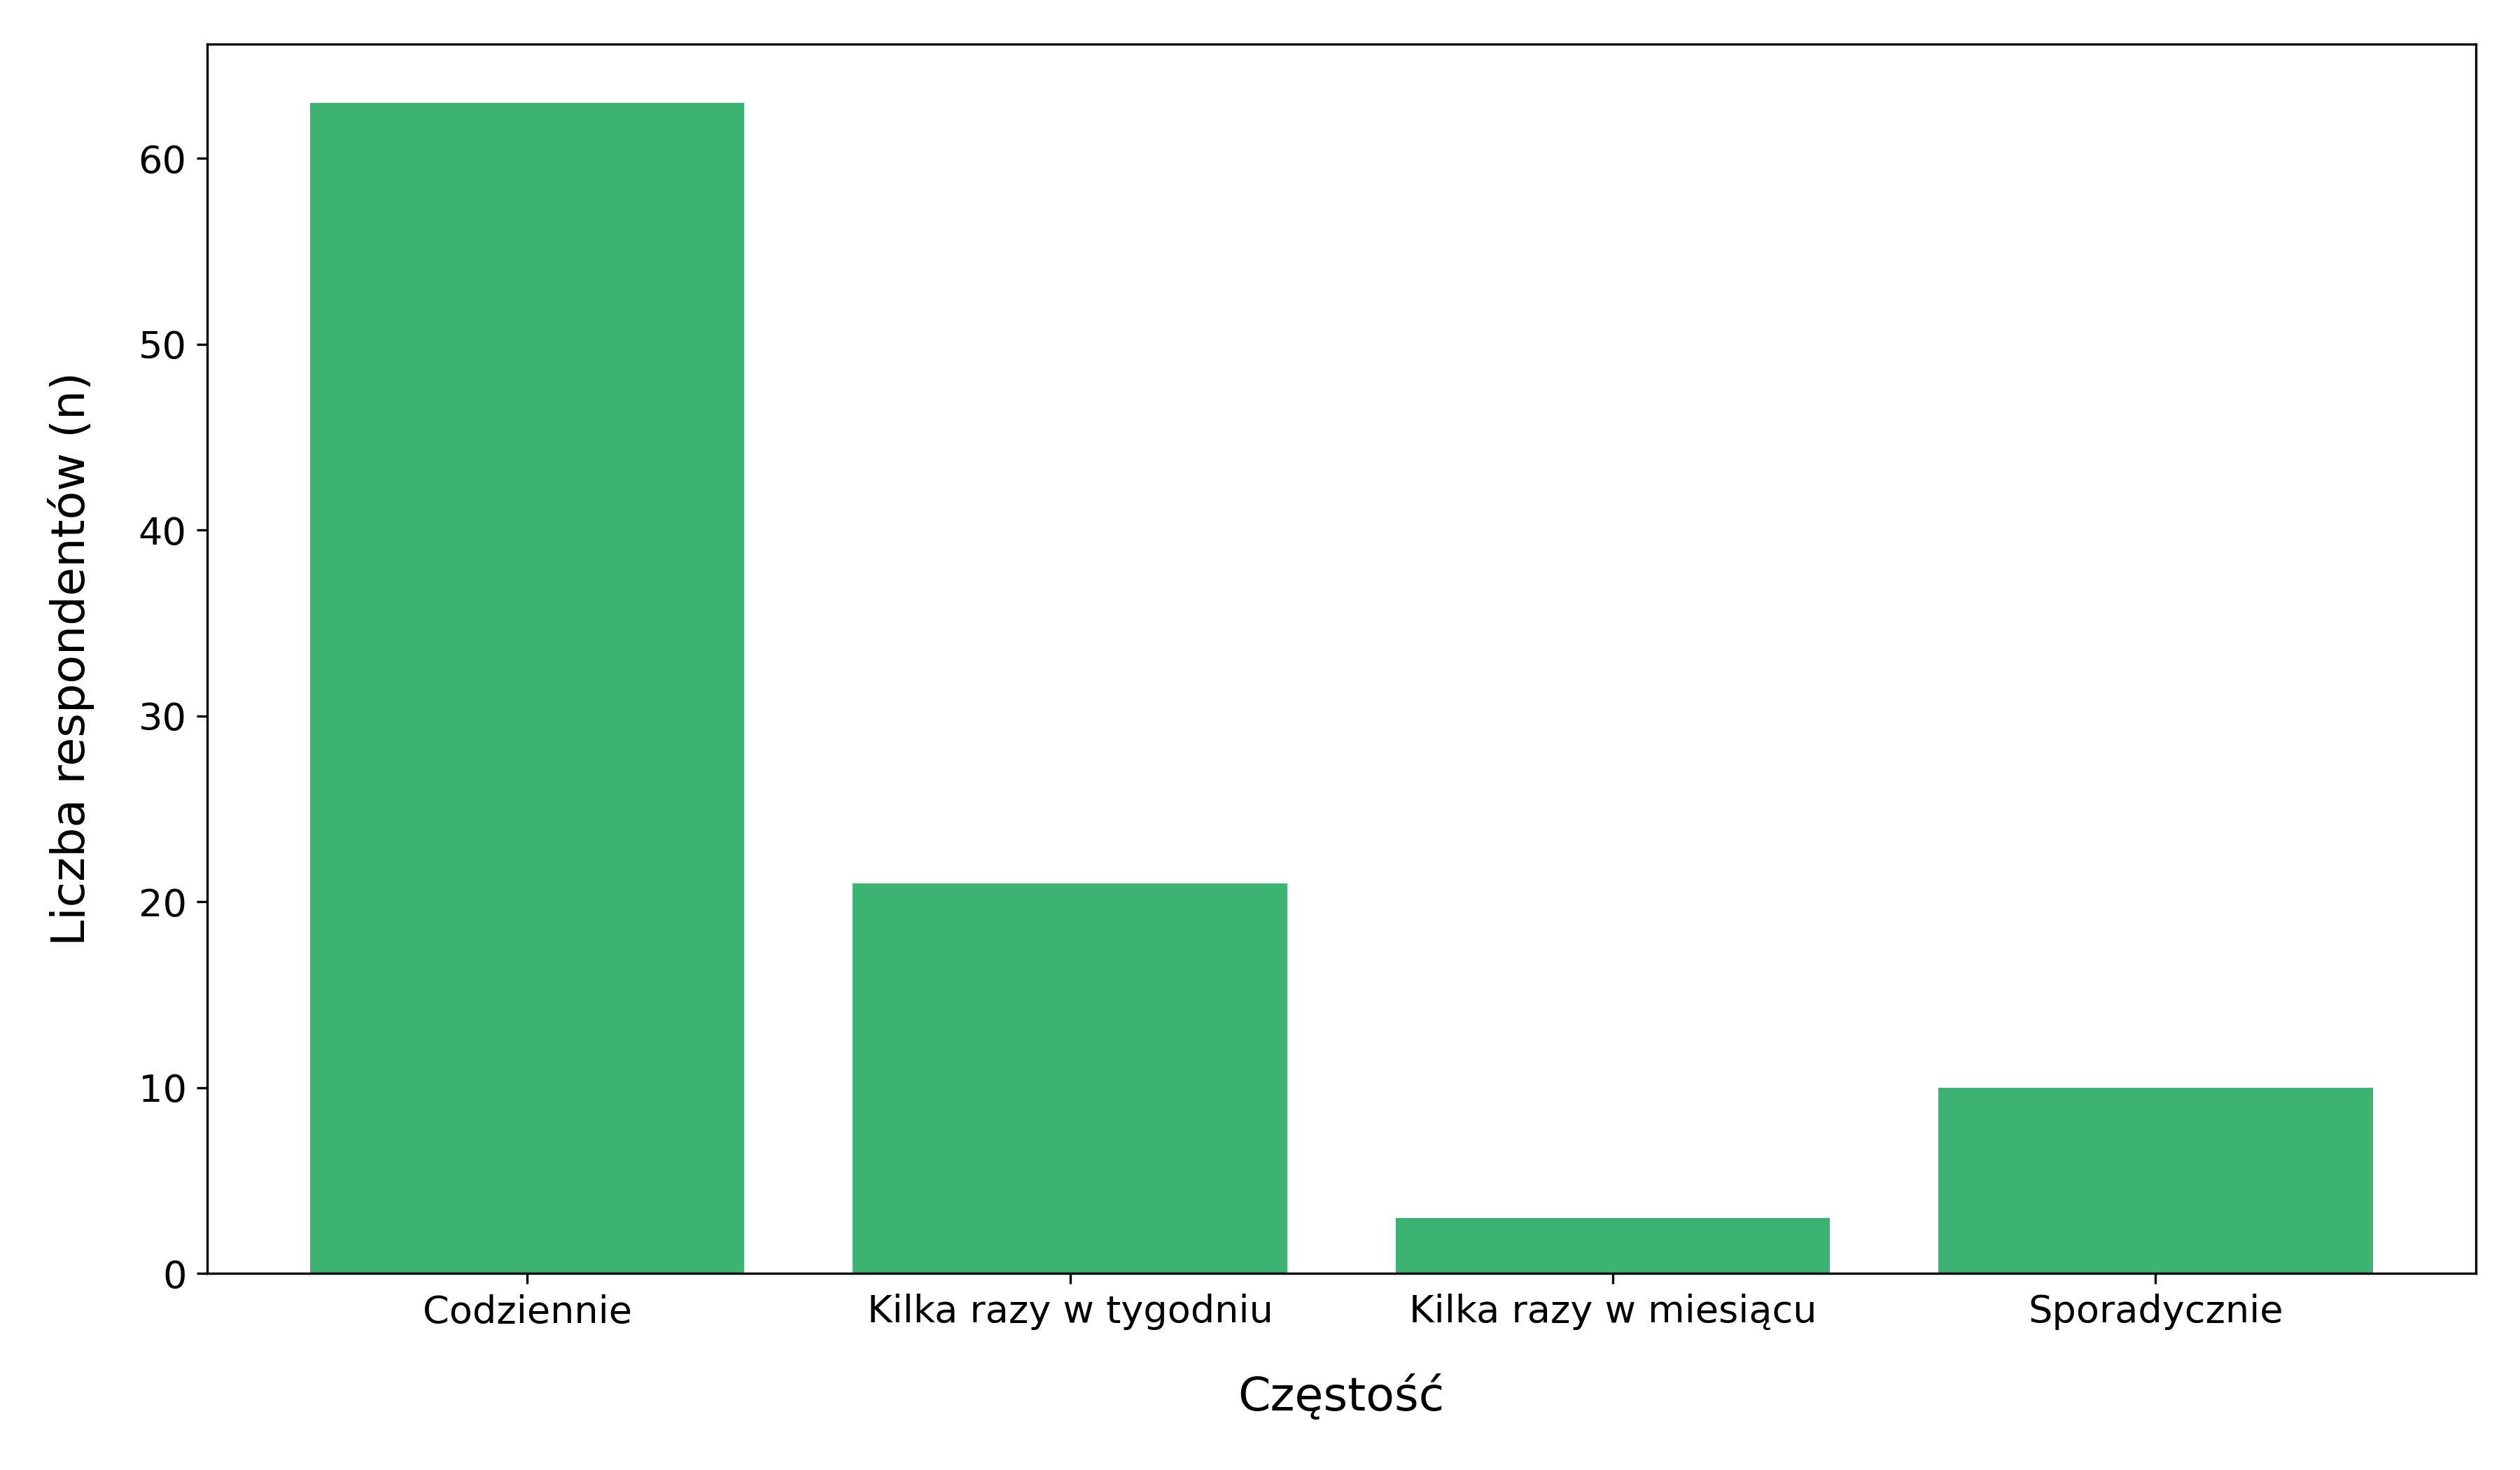
\includegraphics[width=\textwidth]{plots/czestosc-suplementow.png}
    \centering
    \caption{Wykres słupkowy pokazujący częstość stosowania suplementów w grupie badawczej.}
    \label{fig:cze-stos-supl}
\end{figure}

% Czas stosowania suplementów

\begin{table}[h!]
    \centering
    \caption{Czas stosowanie suplementów}
    \label{tab:czas-stos-supl}
    \begin{tabular}{|l|l|l|}
        \hline
        Czas stosowania & n & \% \\
        \hline
        \hline
        < 3 miesięcy & 15 & 15.46 \\
        \hline
        3–12 miesięcy & 23 & 23.71 \\
        \hline
        1–3 lata & 22 & 22.68 \\
        \hline
        >3 lat & 37 & 38.15 \\
        \hline
    \end{tabular}
\end{table}

\begin{figure}
    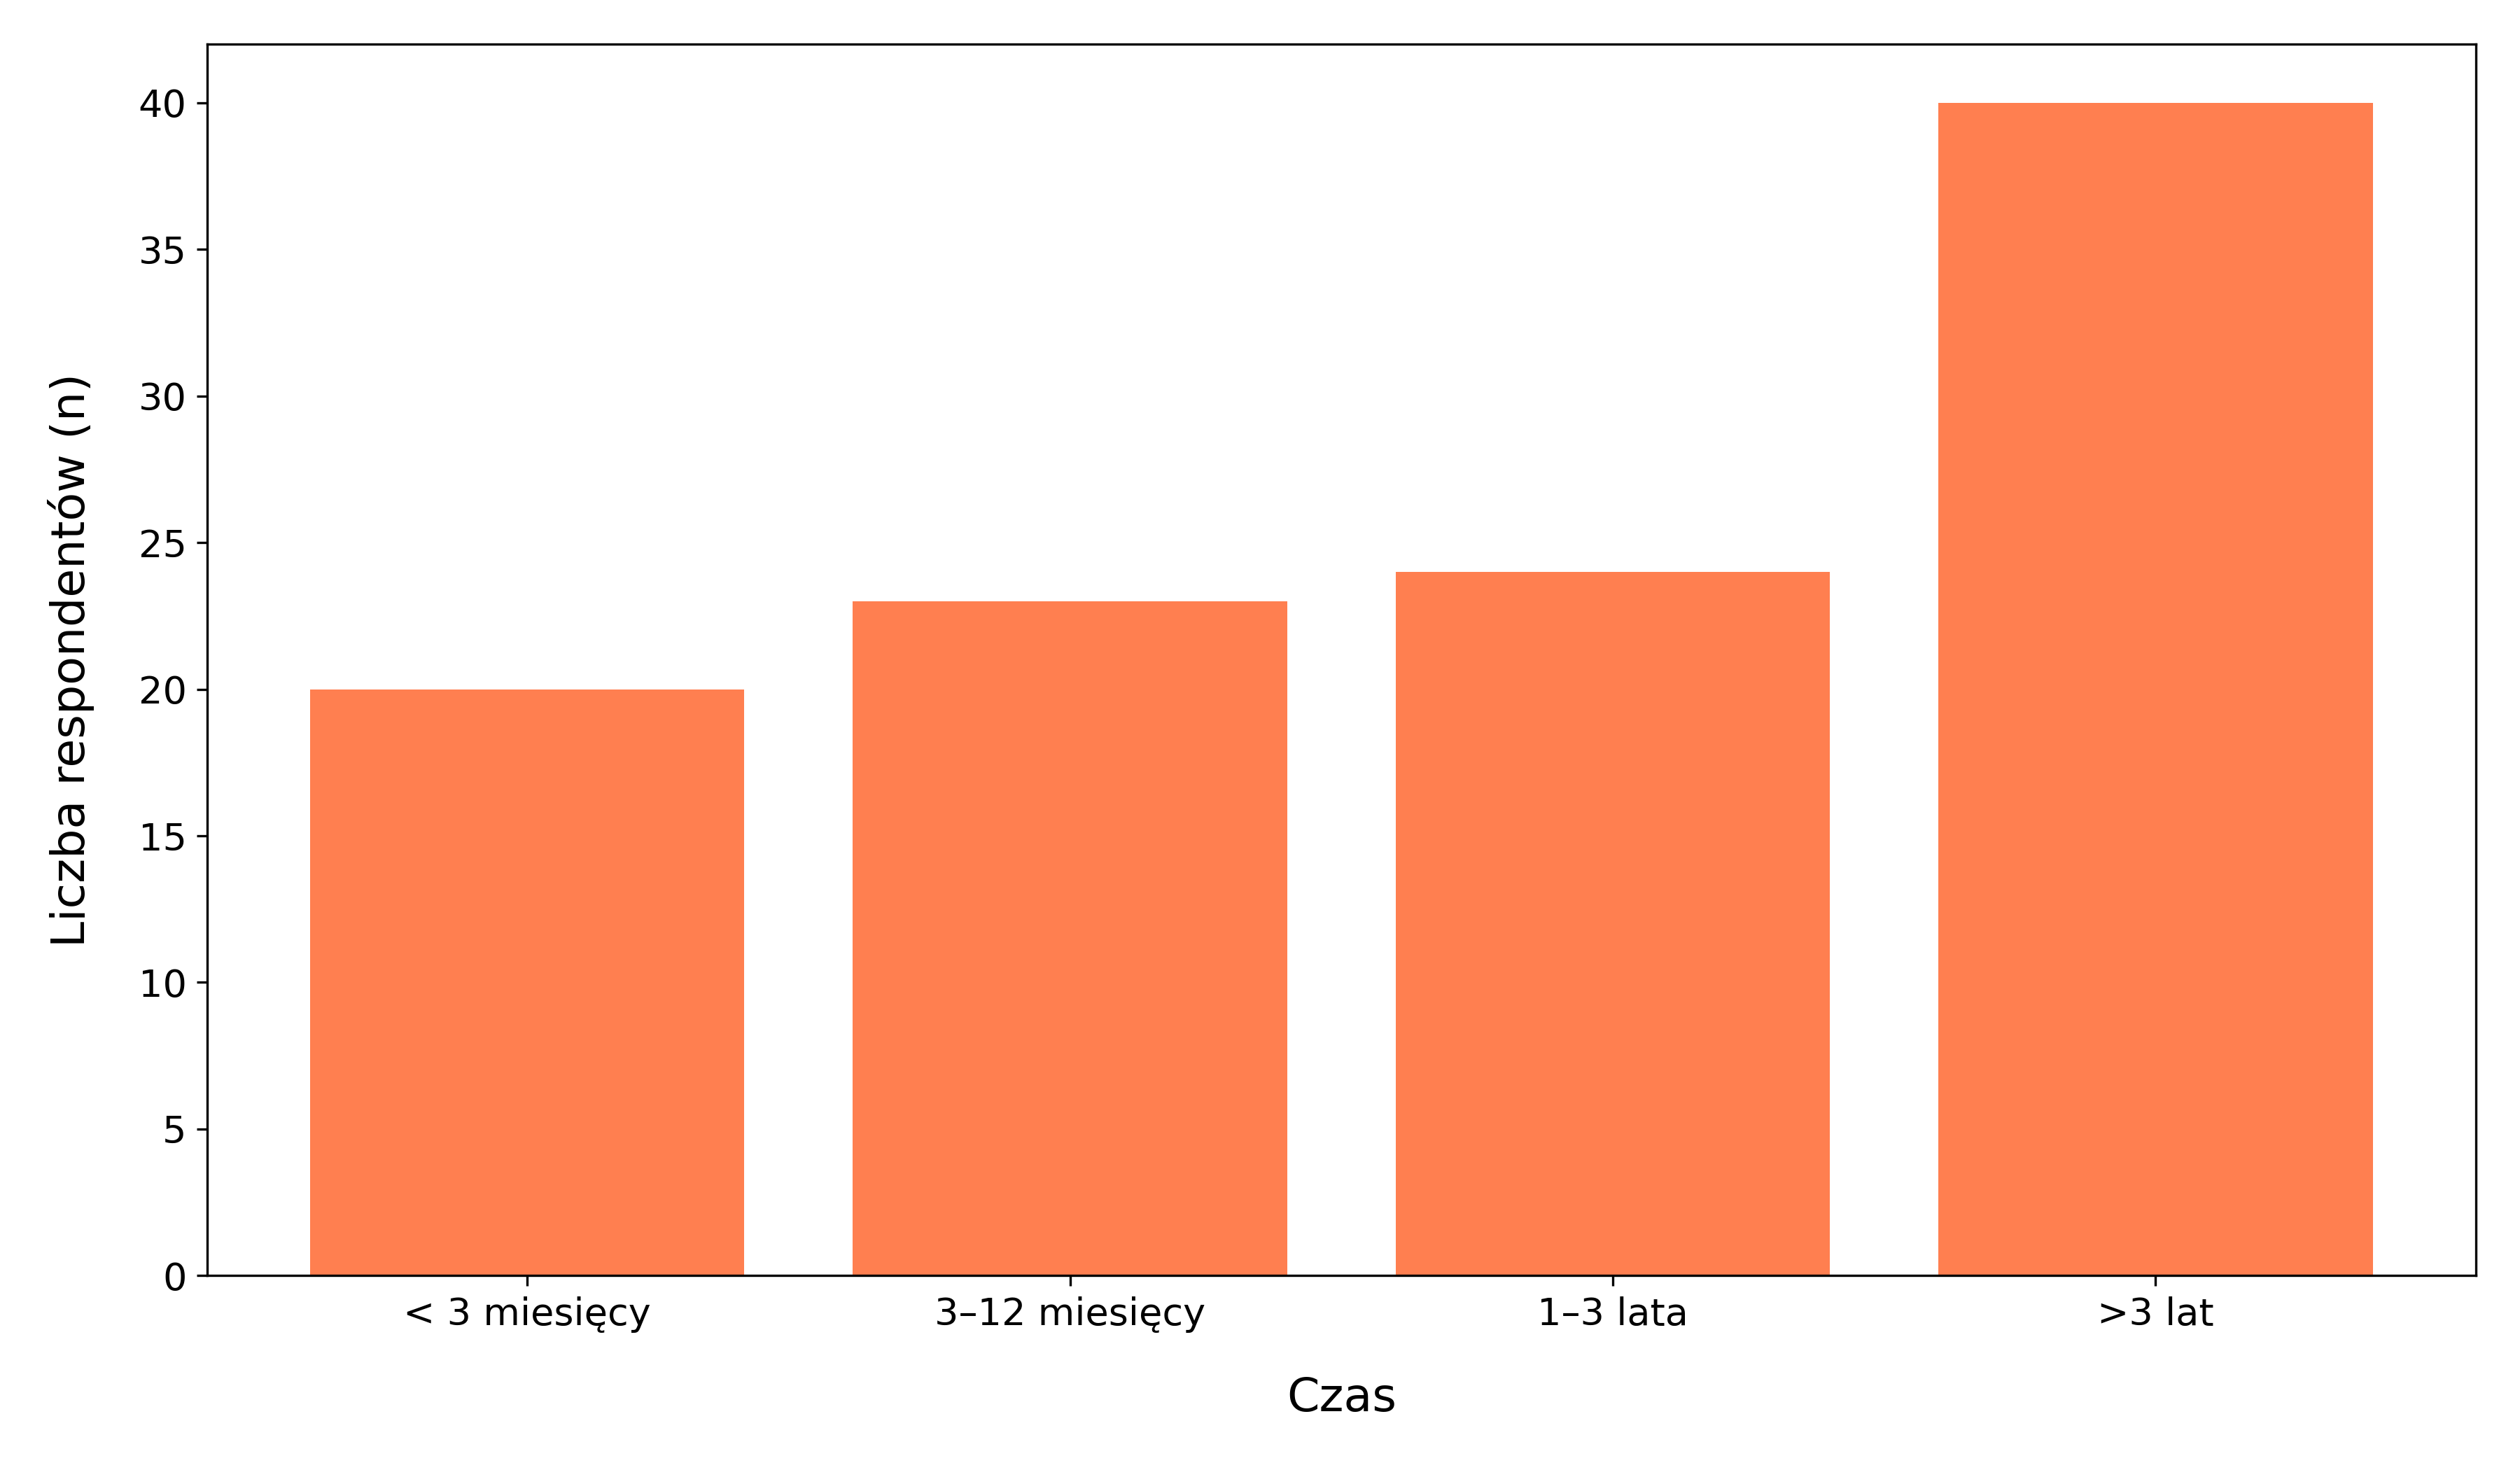
\includegraphics[width=\textwidth]{plots/czas-suplementow.png}
    \centering
    \caption{Wykres słupkowy pokazujący czas stosowania suplementów w grupie badawczej.}
    \label{fig:czas-stos-supl}
\end{figure}

% Wykres słupkowy pokazujący odsetek osób stosujących i niestosujących suplementów.
% Dodatkowo
% Wśród osób stosujących suplementy należy opisać:
%     + jak często je stosują,
%     + od jak dawna je stosują.

% Statystyka
% Statystyka opisowa:
%     + n,
%     + %.
% Można później wykorzystać zmienną „stosowanie suplementów: tak/nie” do analiz zależności.

\subsection{Rodzaje stosowanych suplementów}

% To pytanie wielokrotnego wyboru, więc procenty należy liczyć względem liczby osób stosujących suplementy, a nie względem wszystkich odpowiedzi.
% Należy pokazać, które suplementy były wybierane najczęściej.

% Wykres
% Najlepszy będzie poziomy wykres słupkowy - ranking suplementów od najczęściej do najrzadziej wybieranych.

% Najczęściej stosowane suplementy

\begin{table}[h!]
    \centering
    \caption{Rodzaje stosowanych suplementów}
    \label{tab:rodz-stos-supl}
    \begin{tabular}{|l|l|l|}
        \hline
        Rodzaj suplementu & n  & \% respondentów \\
        \hline
        \hline
        Witamina D & 79 & 81.4 \\
        \hline
        Kwasy omega-3 & 59 & 60.8 \\
        \hline
        Magnez & 48 & 49.4 \\
        \hline
        Probiotyki & 40 & 41.2 \\
        \hline
        Inne odpowiedzi & 39 & 40.2 \\
        \hline
        Multiwitaminy & 32 & 32.9 \\
        \hline
        Witamina C & 31 & 31.9 \\
        \hline
        Białko & 24 & 24.7 \\
        \hline
        Kreatyna & 15 & 15.4 \\
        \hline
        Adaptogeny (np. ashwagandha) & 11 & 11.3 \\
        \hline
    \end{tabular}
\end{table}

\begin{figure}
    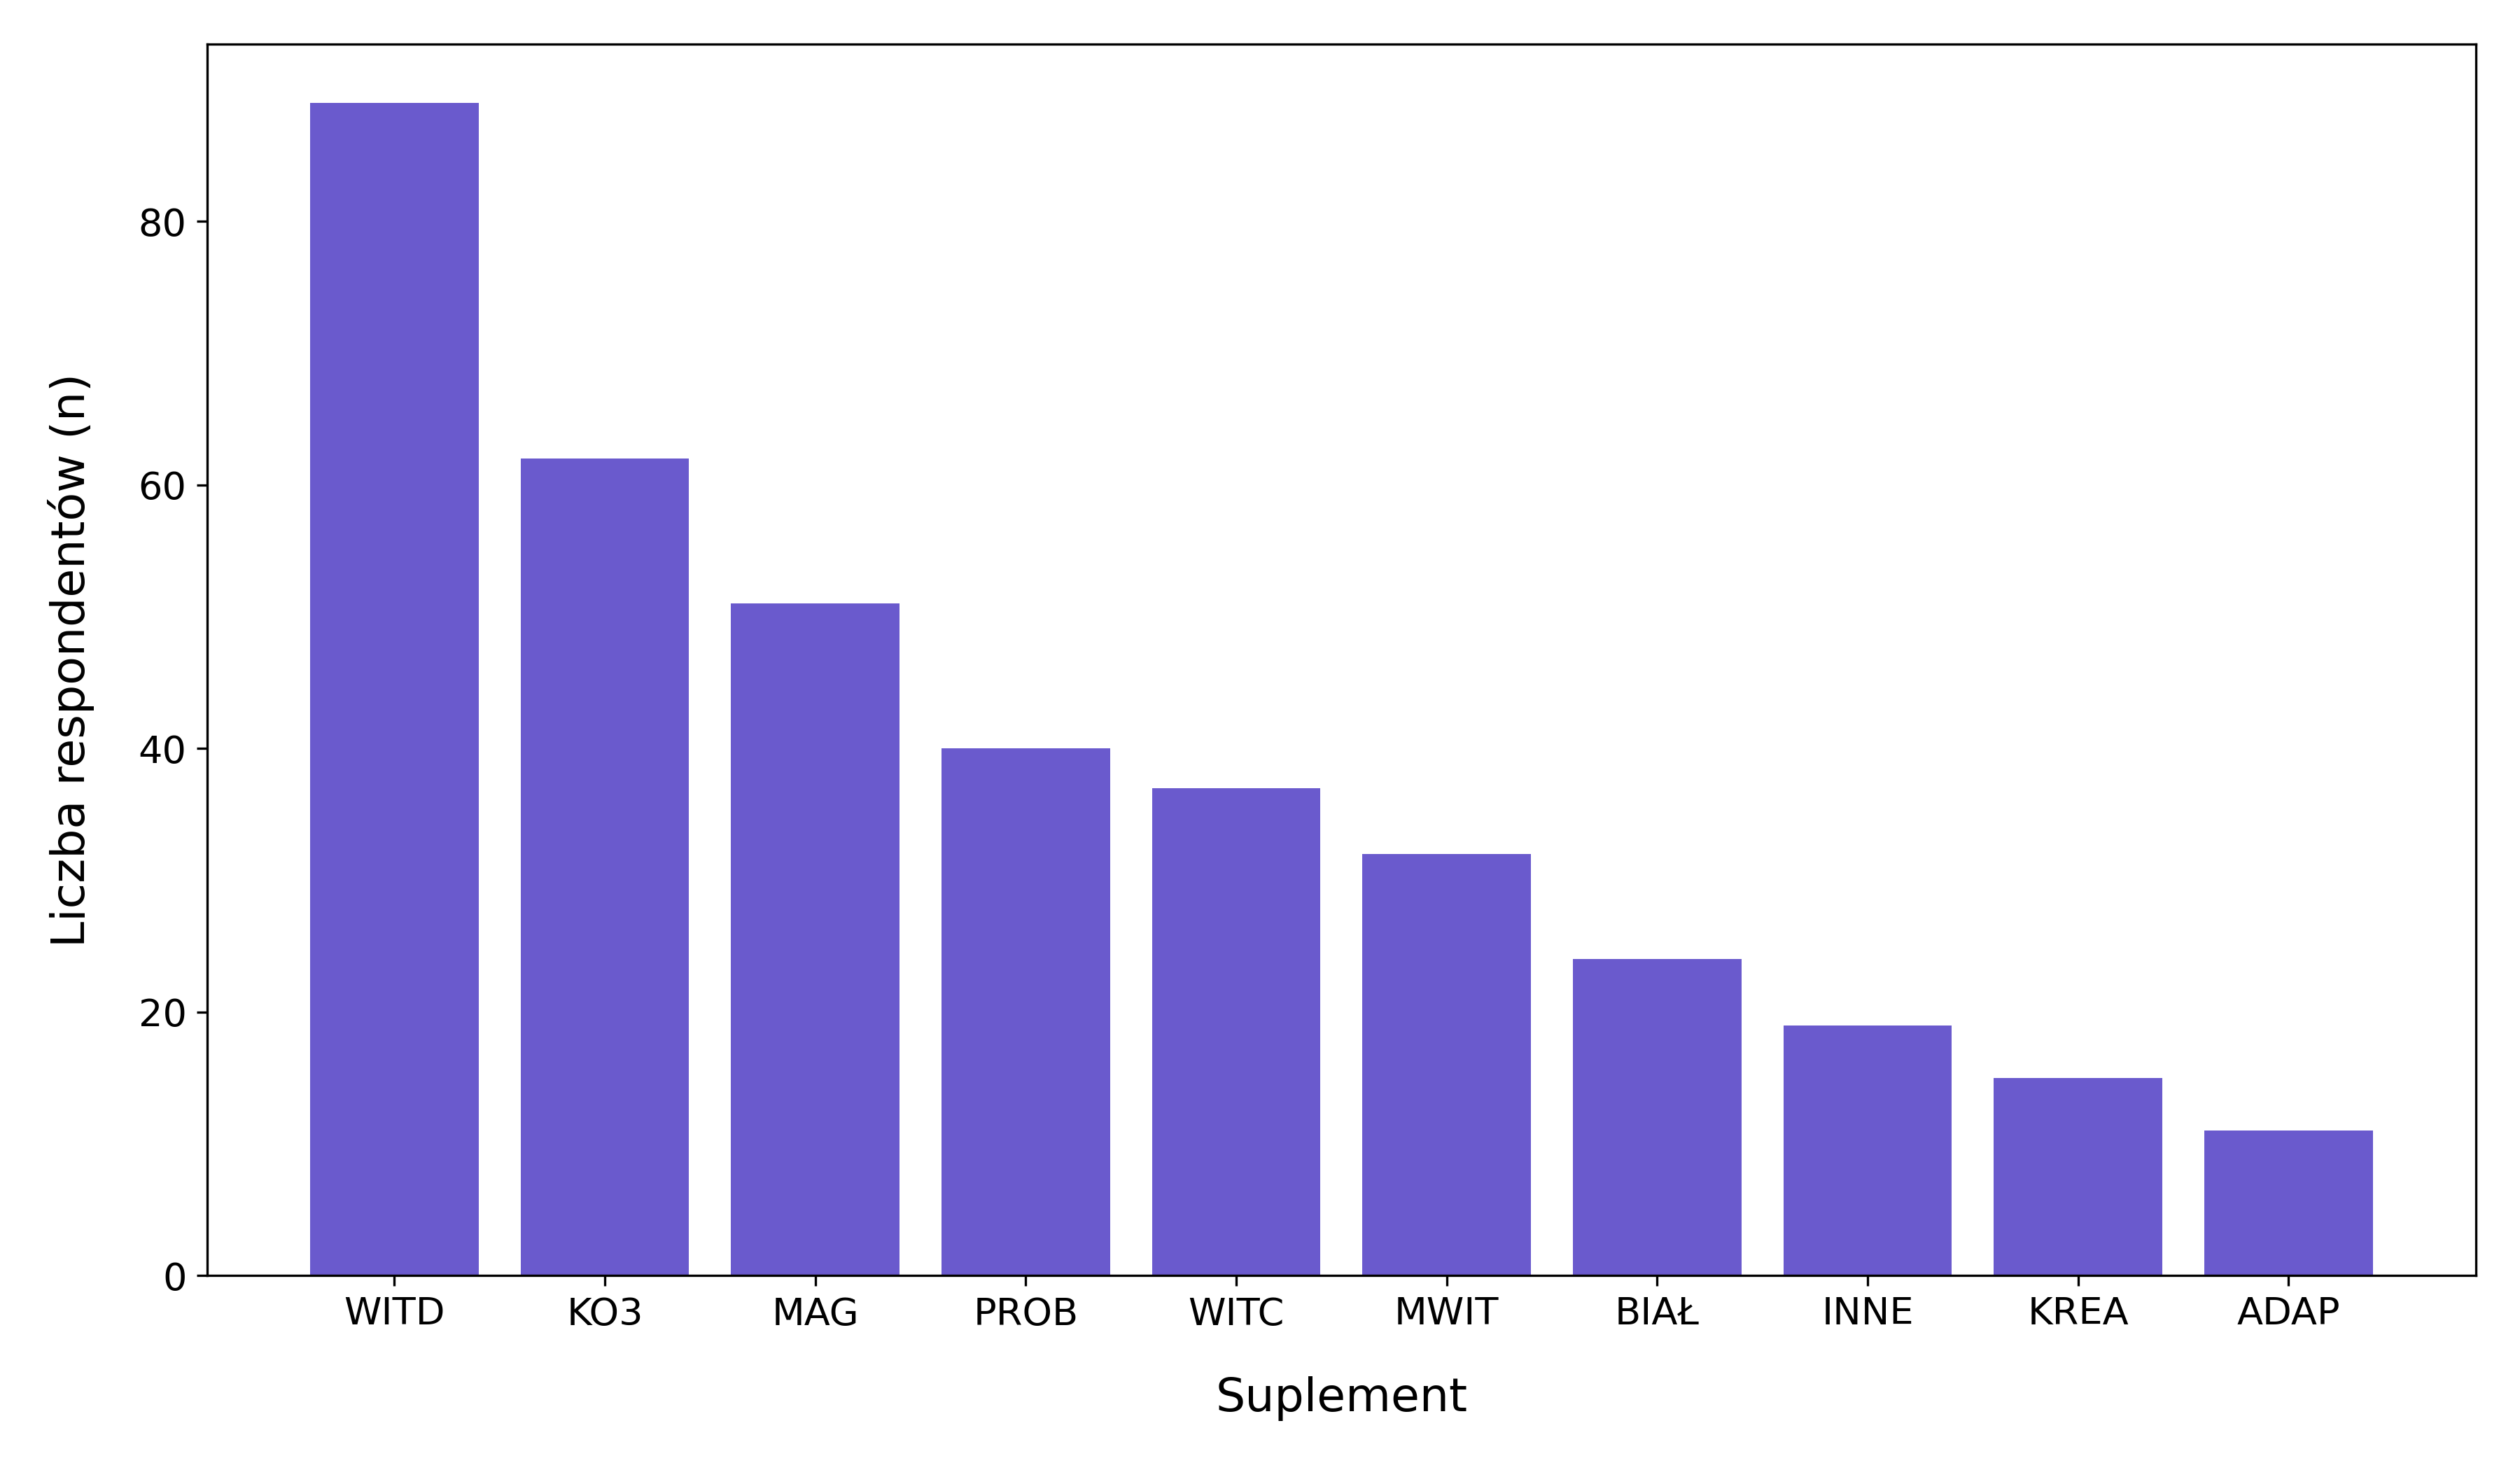
\includegraphics[width=\textwidth]{plots/rodzaje-suplementow.png}
    \centering
    \caption{Wykres słupkowy pokazujący rodzaje stosowanych suplementów w grupie badawczej. Zastosowane skróty: WITD - Witamina D, MAG - Magnez, WITC - Witamina C, MWIT - Multiwitaminy, KO3 - Kwasy omega-3, PROB - Probiotyki, KREA - Kreatyna, BIAŁ - Białko, ADAP - Adaptogeny (np. ashwagandha), INNE - Inne odpowiedzi.}

    \label{fig:rodz-stos-supl}
\end{figure}

% Statystyka
% Statystyka opisowa:
%     + n,
%     + %.

\subsection{Powody suplementacji}

% To również pytanie wielokrotnego wyboru. Procenty liczymy względem liczby osób stosujących suplementy.

% Tabela 6. Powody stosowania suplementów diety
% Powód stosowania, n, % osób stosujących suplementy
% Poprawa zdrowia
%   + Zapobieganie niedoborom
%   + Wzmocnienie odporności
%   + Poprawa wyglądu
%   + Zwiększenie energii
%   + Poprawa koncentracji
%   + Poprawa samopoczucia
%   + Inne

% Powody suplementacji

\begin{table}[h!]
    \centering
    \caption{Powody suplementacji}
    \label{tab:powody-supl}
    \begin{tabular}{|l|l|l|}
        \hline
        Powód stosowania & n  & \% respondentów \\
        \hline
        \hline
        Poprawa zdrowia & 68 & 70.1 \\
        \hline
        Wzmocnienie odporności & 66 & 68.04 \\
        \hline
        Zapobieganie niedoborom & 65 & 67.01 \\
        \hline
        Poprawa samopoczucia & 50 & 51.55 \\
        \hline
        Zwiększenie energii & 49 & 50.52 \\
        \hline
        Poprawa wyglądu (skóra, włosy, paznokcie) & 46 & 47.42 \\
        \hline
        Poprawa koncentracji & 44 & 45.36 \\
        \hline
        Inne odpowiedzi & 4  & 4.12 \\
        \hline
    \end{tabular}
\end{table}

\begin{figure}
    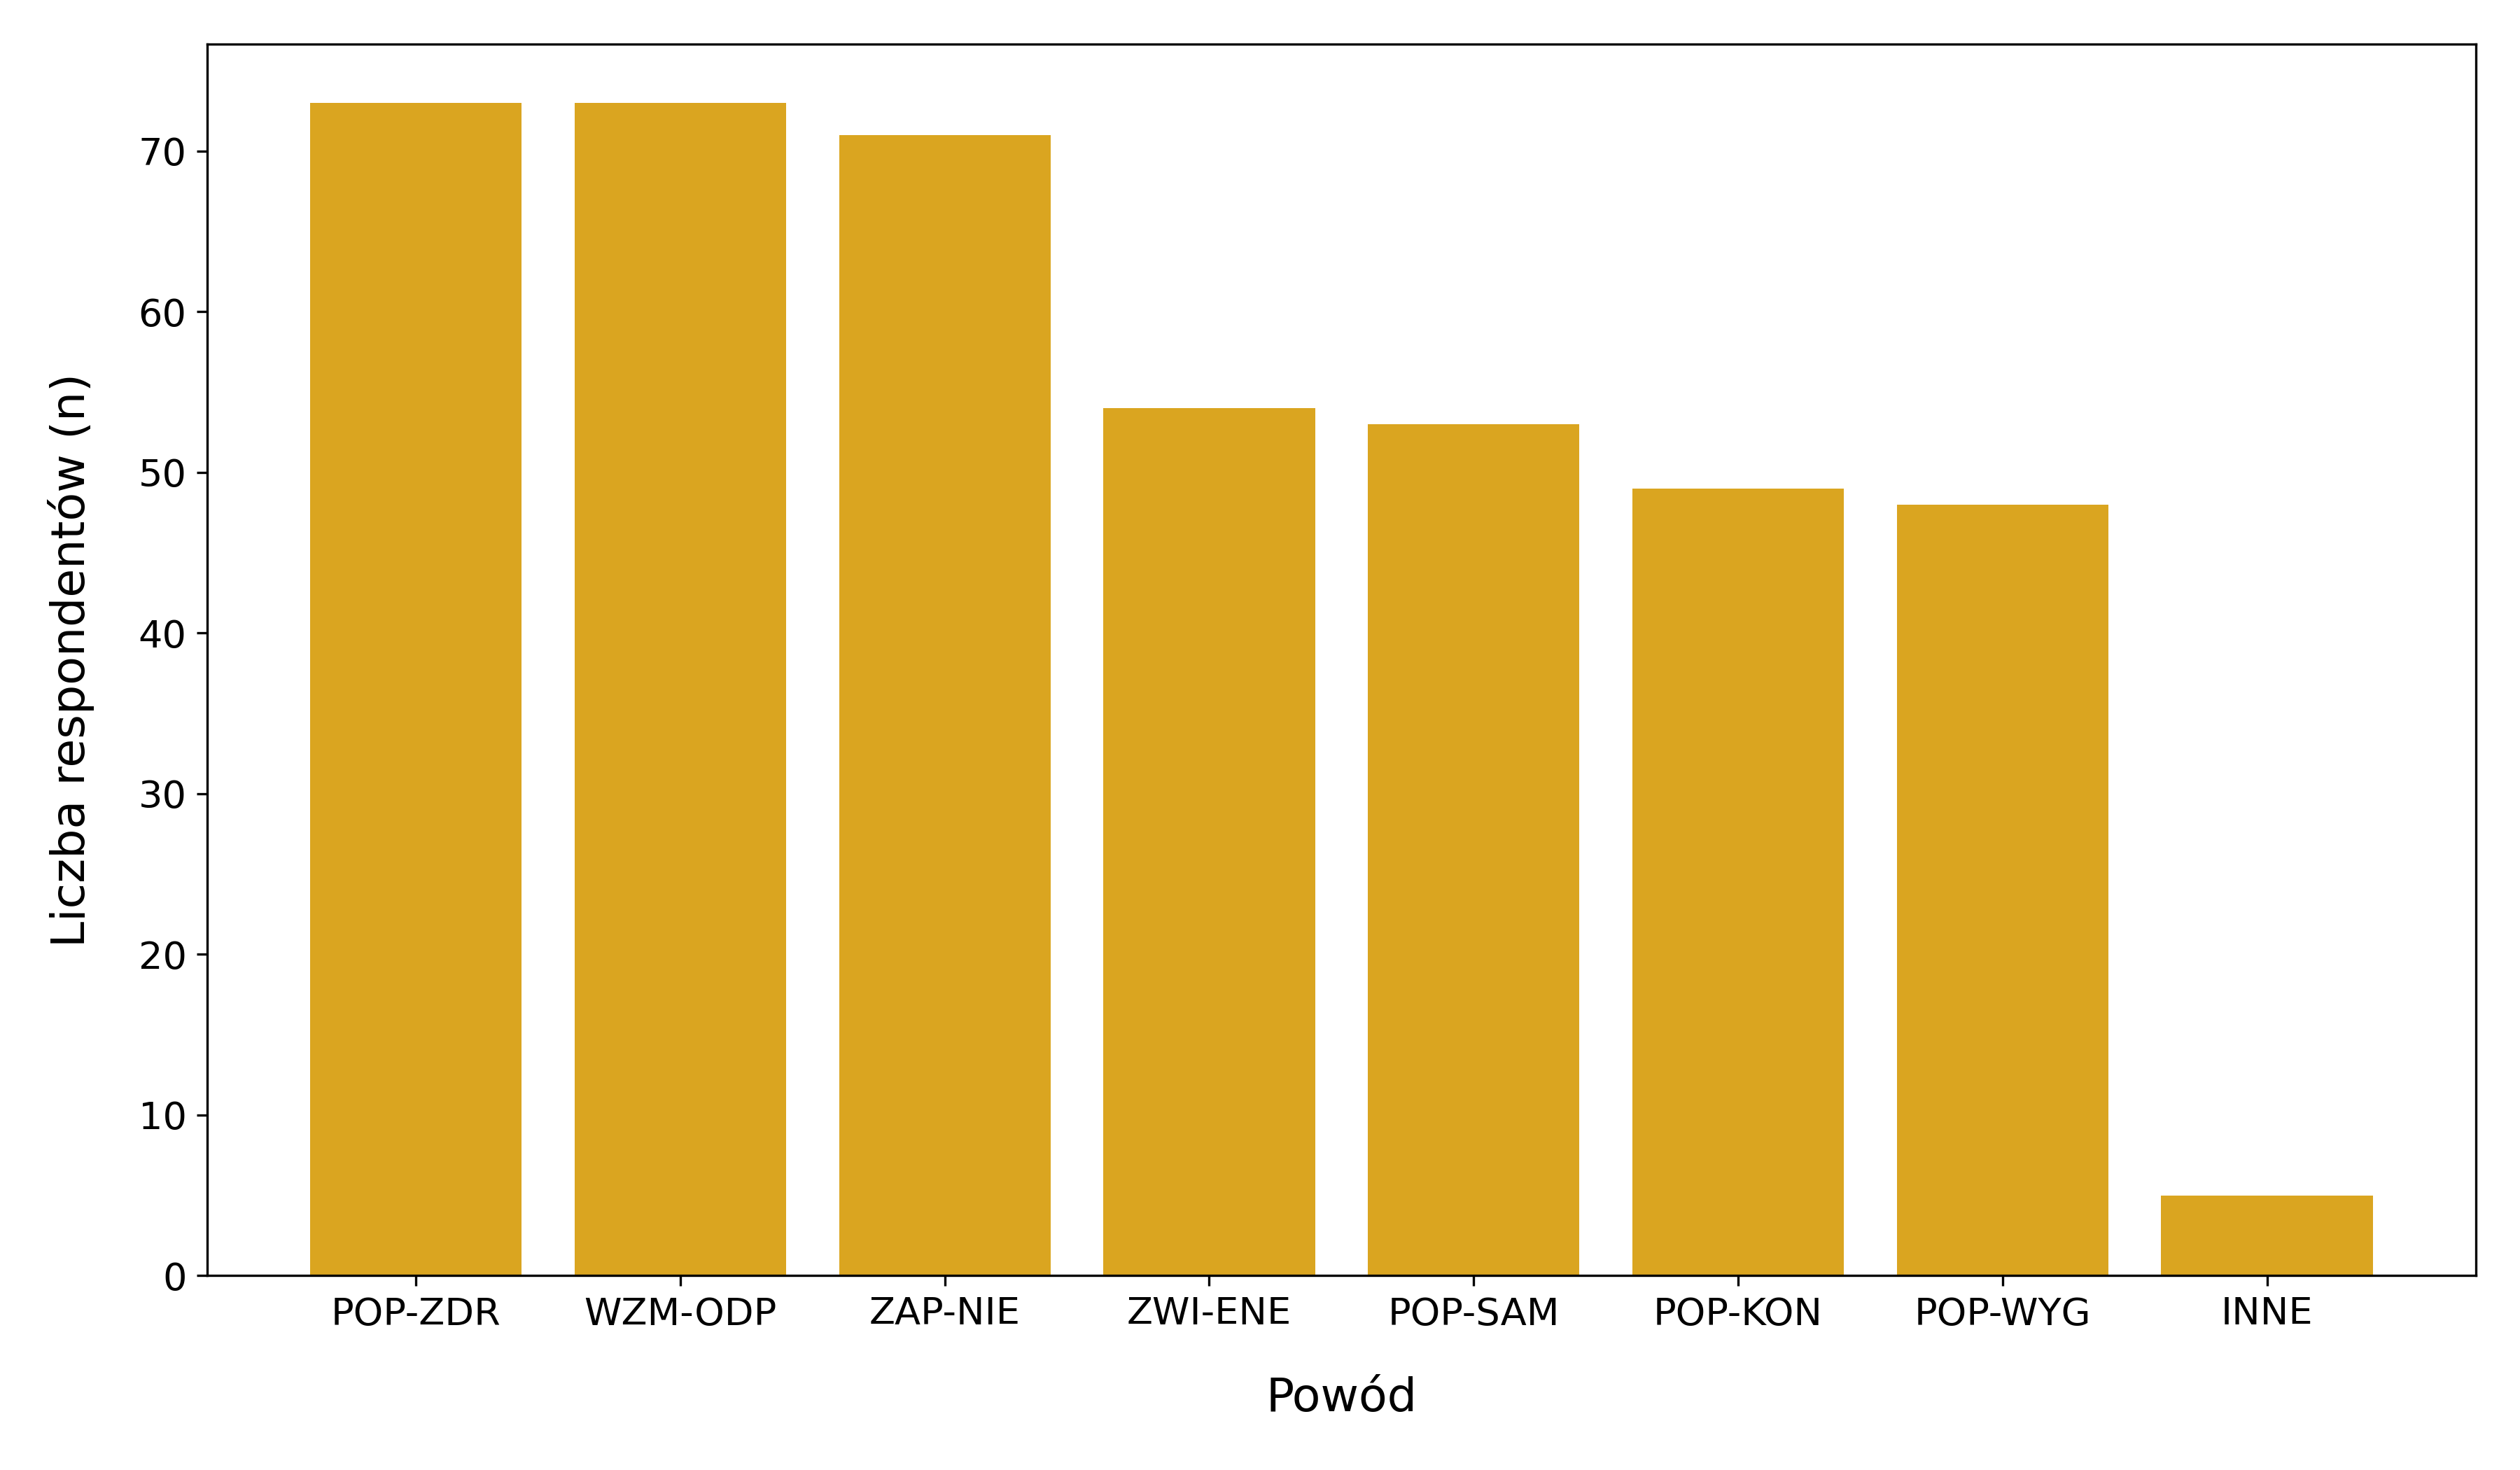
\includegraphics[width=\textwidth]{plots/powody-suplementacji.png}
    \centering
    \caption{Wykres słupkowy pokazujący powody suplementacji w grupie badawczej. Zastosowane skróty: POPZDR - Poprawa zdrowia, ZAPNIE - Zapobieganie niedoborom, WZMODP - Wzmocnienie odporności, POPWYG - Poprawa wyglądu (skóra włosy paznokcie), ZWIENE - Zwiększenie energii, POPKON - Poprawa koncentracji, POPSAM - Poprawa samopoczucia, INNE - Inne odpowiedzi.}
    \label{fig:powody-supl}
\end{figure}

% Wykres
% Poziomy wykres słupkowy - ranking powodów suplementacji.
% Statystyka
% Opisowo:
%     + n,
%     + %.

\subsection{Źródła wiedzy}

% Należy pokazać, skąd studenci czerpią wiedzę o suplementach.

% Źródła

\begin{table}[h!]
    \centering
    \caption{Źródła informacji}
    \label{tab:zrodla-info}
    \begin{tabular}{|l|l|l|}
        \hline
        Źródło & n  & \% respondentów \\
        \hline
        \hline
        Internet (artykuły, blogi) & 67 & 69.07 \\
        \hline
        Lekarz & 39 & 40.21 \\
        \hline
        Dietetyk & 37 & 38.14 \\
        \hline
        Media społecznościowe  & 31 & 31.96 \\
        \hline
        Znajomi/rodzina & 29 & 29.9 \\
        \hline
        Farmaceuta & 27 & 27.84 \\
        \hline
        Reklamy & 10 & 10.31 \\
        \hline
        Inne odpowiedzi & 10  & 10.31 \\
        \hline
    \end{tabular}
\end{table}

\begin{figure}
    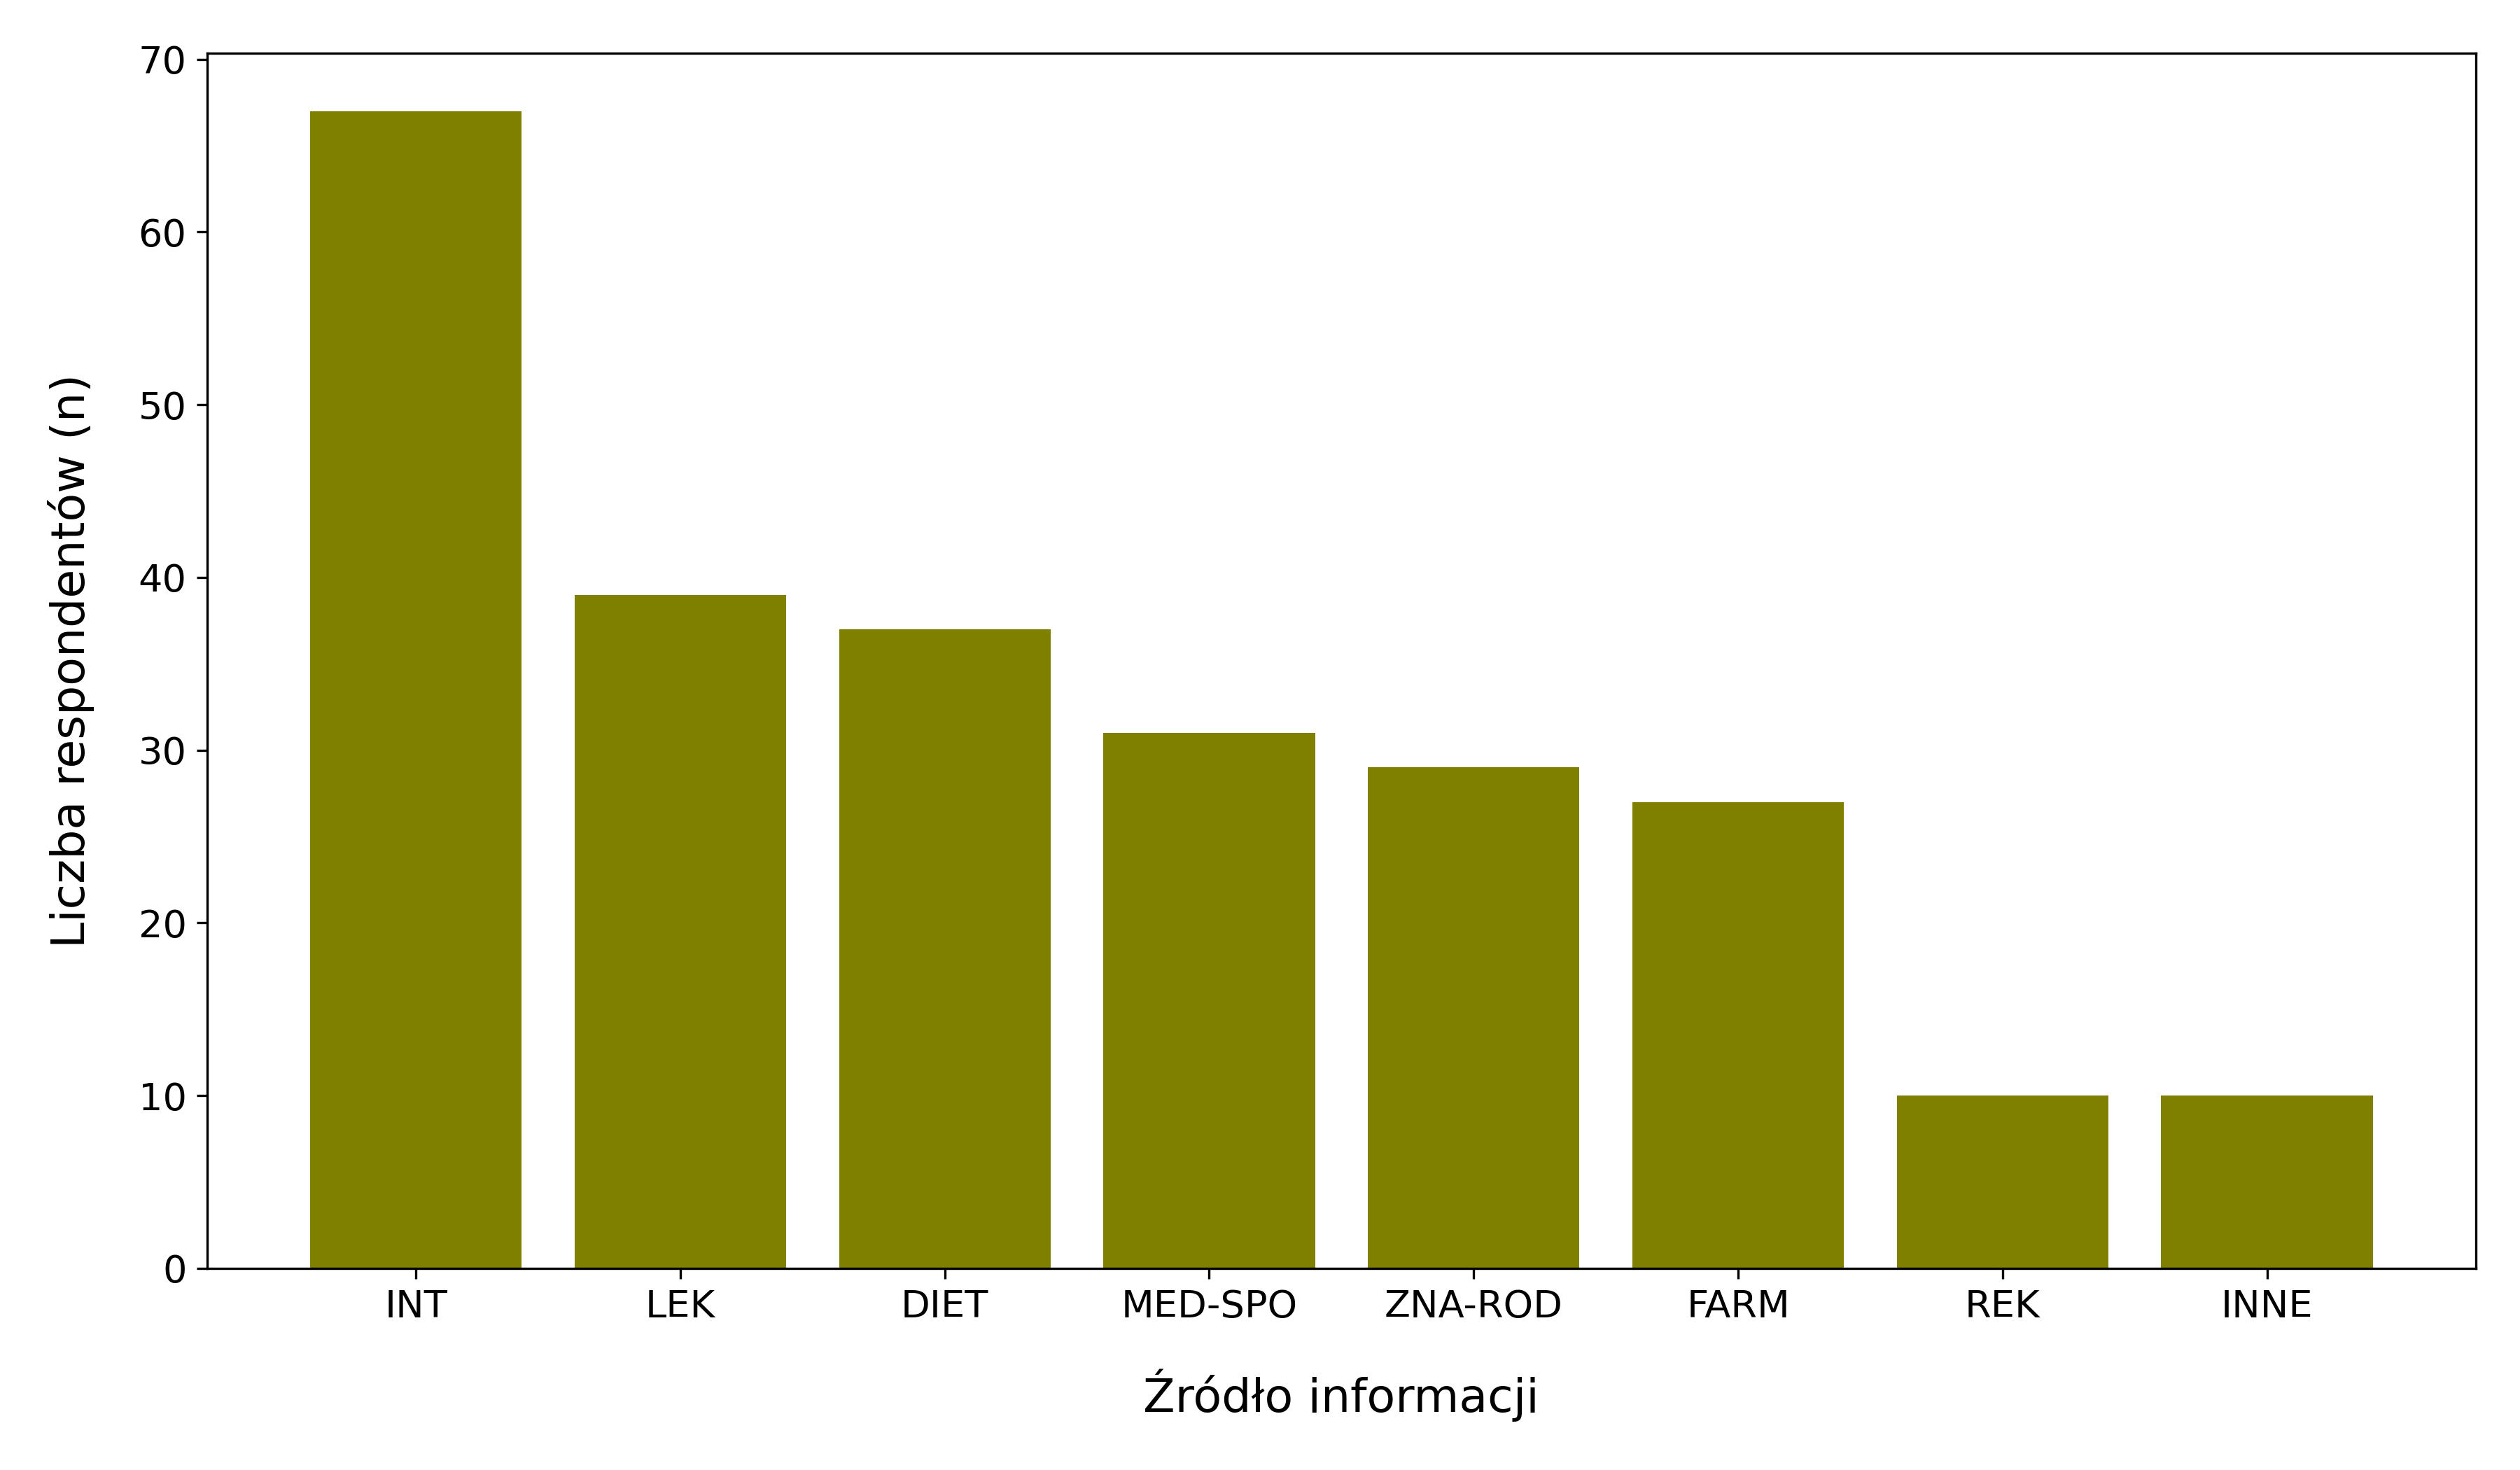
\includegraphics[width=\textwidth]{plots/zrodla-informacji.png}
    \centering
    \caption{Wykres pokazujący źródła informacji o suplementach w grupie badawczej. Zastosowane skróty: INT - Internet (artykuły, blogi), LEK - Lekarz, DIET - Dietetyk, MED-SPO - Media społecznościowe, ZNA-ROD - Znajomi/rodzina, FARM - Farmaceuta, REK - Reklamy, INNE - Inne odpowiedzi.}
    \label{fig:zrodla-info}
\end{figure}

% Wiarygodne źródła

\begin{table}[h!]
    \centering
    \caption{Wiarygodne źródła informacji. Zastosowane skróty: PROF - \enquote{Takie, którego polecenia nie wynikają z profitów jakie otrzymują}, FUNK - \enquote{Lekarze medycyny funkcjonalnej}, ZBR - \enquote{Portale zbierające wyniki badań lub też oponie specjalistów, ale wielu, żeby mozna było porównać podejścia, nie ufam jednemu lekarzowi, dietetykowi itp. ponieważ każdy mówi co innego}.}
    \label{tab:wiarygodne-zrodla}
    \begin{tabular}{|l|l|l|}
        \hline
        Źródło & n  & \% respondentów \\
        \hline
        \hline
        Lekarz & 67 & 69.07 \\
        \hline
        Naukowe portale internetowe & 39 & 40.21 \\
        \hline
        Instytucje zdrowia publicznego & 37 & 38.14 \\
        \hline
        Dietetyk & 31 & 31.96 \\
        \hline
        Farmaceuta & 29 & 29.9 \\
        \hline
        Badania naukowe & 27 & 27.84 \\
        \hline
        PROF & 10 & 10.31 \\
        \hline
        FUNK & 10  & 10.31 \\
        \hline
        ZBR & 10  & 10.31 \\
        \hline
    \end{tabular}
\end{table}

\begin{figure}
    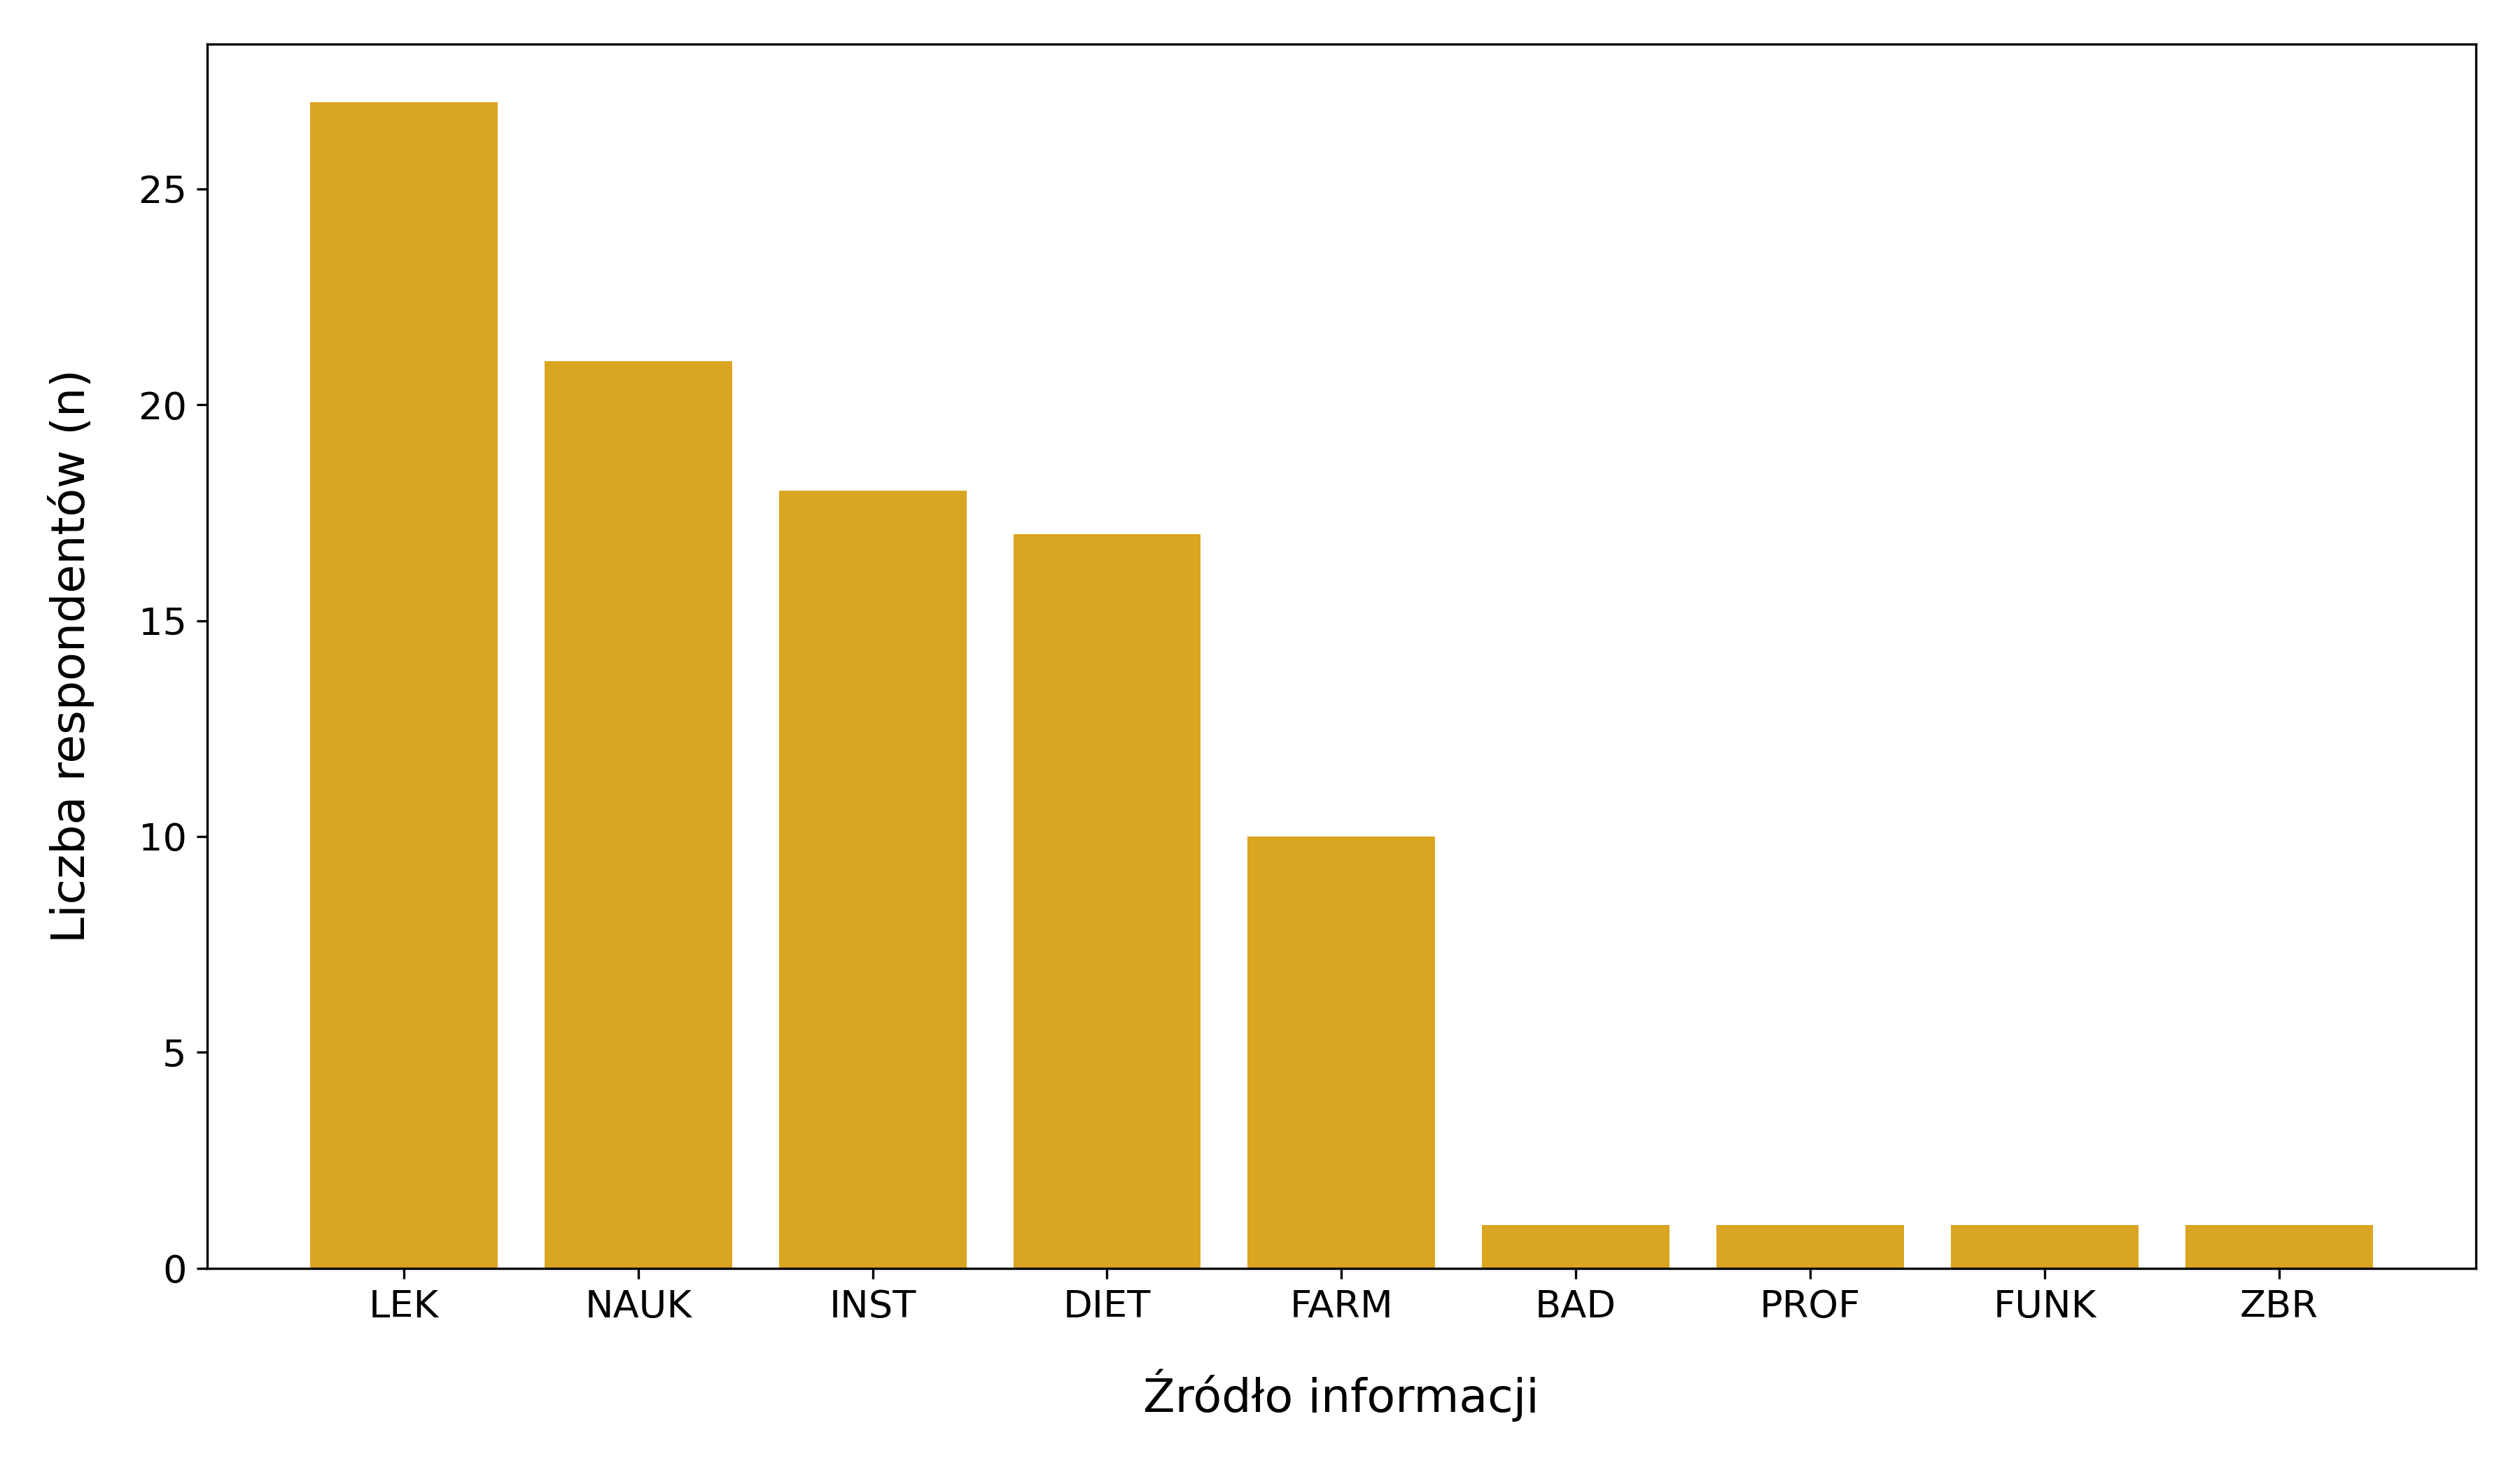
\includegraphics[width=\textwidth]{plots/wiarygodne-zrodla.png}
    \centering
    \caption{Wykres pokazujący zaufanie w różne źródła informacji o suplementach w grupie badawczej. Zastosowane skróty: LEK - Lekarz, NAUK - Naukowe portale internetowe, INST - Instytucje zdrowia publicznego, DIET - Dietetyk, FARM - Farmaceuta, BAD - Badania naukowe, PROF - \enquote{Takie, którego polecenia nie wynikają z profitów jakie otrzymują}, FUNK - \enquote{Lekarze medycyny funkcjonalnej}, ZBR - \enquote{Portale zbierające wyniki badań lub też oponie specjalistów, ale wielu, żeby mozna było porównać podejścia, nie ufam jednemu lekarzowi, dietetykowi itp. ponieważ każdy mówi co innego}.}
    \label{fig:wiarygodne-zrodla}
\end{figure}

% Preferowane formy edukacji

\begin{table}[h!]
    \centering
    \caption{Preferowane formy edukacji}
    \label{tab:formy}
    \begin{tabular}{|l|l|l|}
        \hline
        Forma & n  & \% respondentów \\
        \hline
        \hline
        Krótkie filmy edukacyjne & 53 & 54.64 \\
        \hline
        Artykuły popularnonaukowe & 45 & 46.39 \\
        \hline
        Warsztaty na uczelni & 39 & 40.21 \\
        \hline
        Infografiki & 32 & 32.99 \\
        \hline
        Konsultacje z farmaceutą & 32 & 32.99 \\
        \hline
        Posty na Instagramie/TikToku & 32 & 32.99 \\
        \hline
        Podcasty & 29 & 29.9 \\
        \hline
        Inne odpowiedzi & 5 & 5.15 \\
        \hline
    \end{tabular}
\end{table}

\begin{figure}
    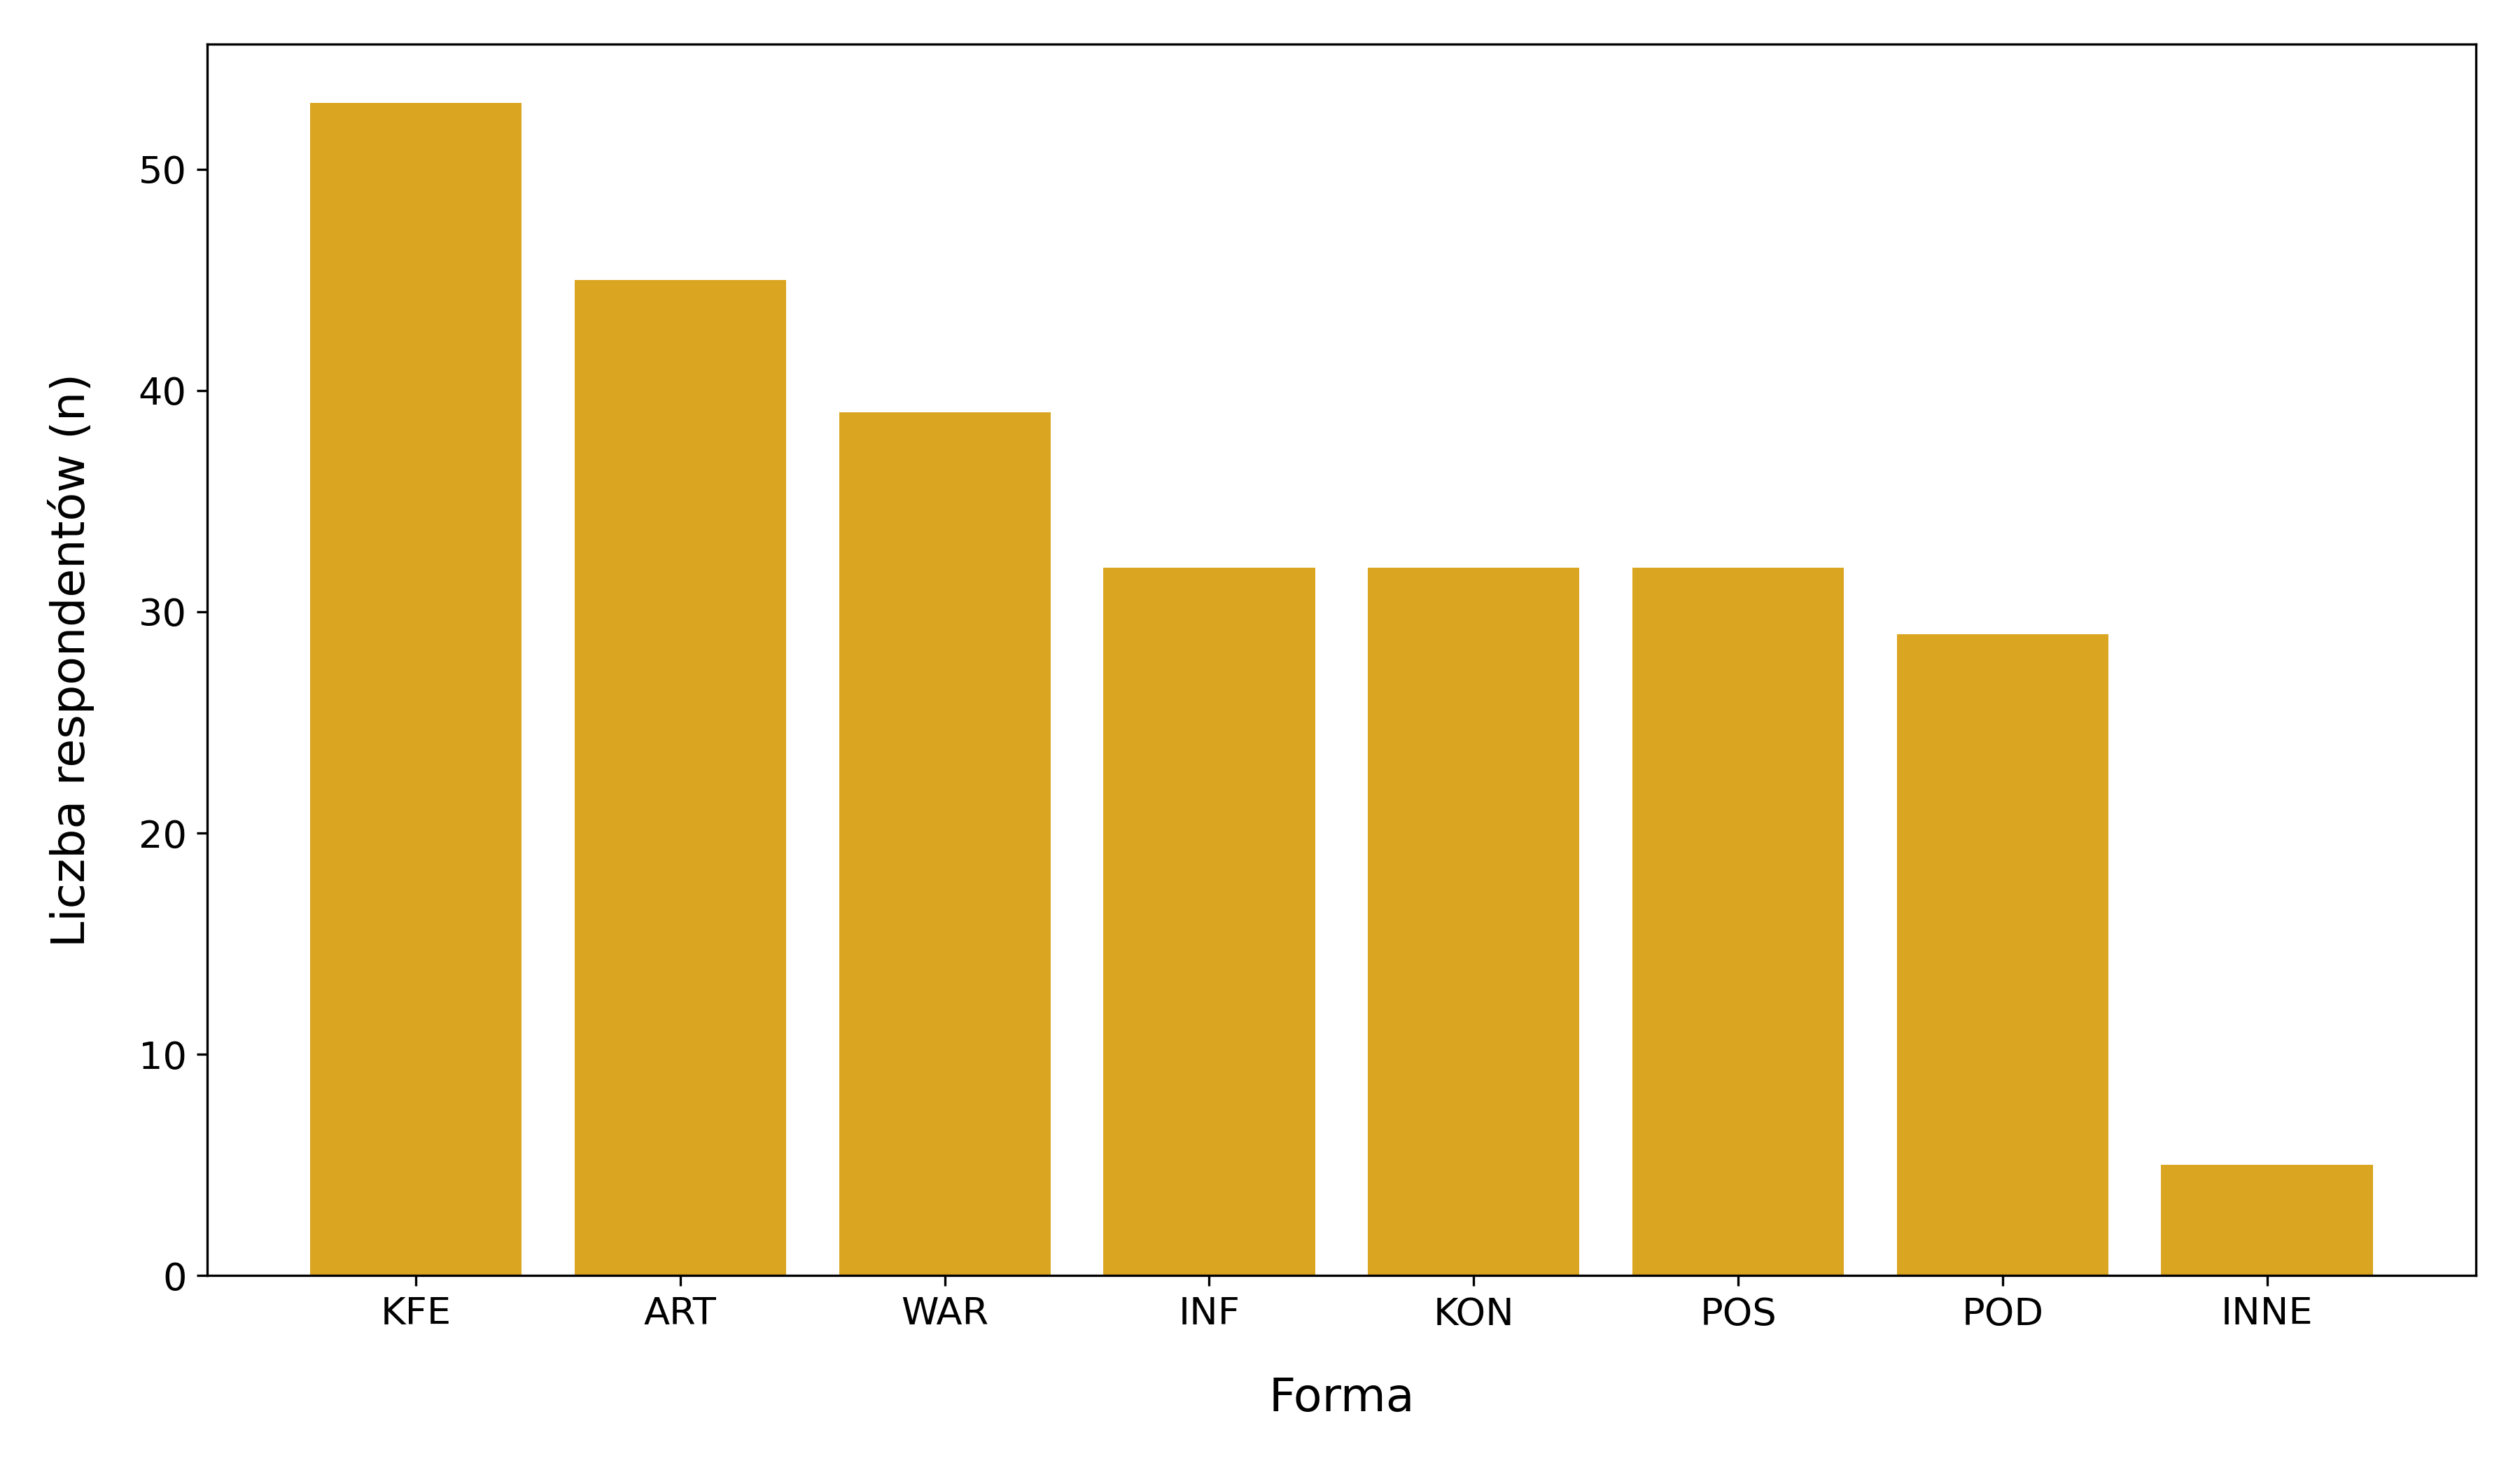
\includegraphics[width=\textwidth]{plots/preferowane-zrodla.png}
    \centering
    \caption{Wykres pokazujący preferowane formy edukacji o suplementach w grupie badawczej. Zastosowane skróty: KFE - Krótkie filmy edukacyjne, ART - Artykuły popularnonaukowe, WAR - Warsztaty na uczelni, INF - Infografiki, KON - Konsultacje z farmaceutą, POS - Posty na Instagramie/TikToku, POD - Podcasty, INNE - Inne odpowiedzi.}
    \label{fig:formy}
\end{figure}

% Tabela 7. Źródła informacji o suplementach diety
% Źródło informacji, n, %
%     + Internet
%     + Media społecznościowe
%     + Reklamy
%     + Lekarz
%     + Dietetyk
%     + Farmaceuta
%     + Znajomi/rodzina
%     + Inne
% Wykres
% Poziomy wykres słupkowy.


% Statystyka
% Opisowo:
%     + n,
%     + %.
% Można dodatkowo podzielić źródła na dwie grupy:
% Źródła profesjonalne
%     + lekarz,
%     + dietetyk,
%     + farmaceuta,
%     + instytucje zdrowia publicznego.
% Źródła nieprofesjonalne
%     + Internet,
%     + media społecznościowe,
%     + reklamy,
%     + znajomi/rodzina.

\subsection{Praktyki suplementacyjne}

% To bardzo ważny podrozdział, ponieważ pokazuje, czy suplementacja jest racjonalna.
% Należy uwzględnić pytania dotyczące:
%     1. przekraczania zalecanych dawek,
%     2. sprawdzania powielania składników,
%     3. wykonywania badań krwi przed suplementacją,
%     4. konsultowania suplementacji ze specjalistą.

% Tabela 8. Praktyki związane z bezpieczeństwem suplementacji
% Praktyka, Odpowiedź, n, %
% Przekraczanie zalecanej dawki, Nigdy / Czasami / Często
% Sprawdzanie powielania składników, Tak / Czasami / Nie
% Badania krwi przed suplementacją, Tak / Częściowo / Nie
% Konsultacja ze specjalistą, Lekarz / Dietetyk / Farmaceuta / Nie

% Statystyka Opisowo:
%     + n,
%     + %.
% Dodatkowo można utworzyć indeks prawidłowych praktyk suplementacyjnych.

\subsection{Indeks prawidłowych praktyk suplementacyjnych}

% Proponuję utworzyć prosty wskaźnik 0–4 punkty.

% Punktacja
% 1. Przekraczanie dawek
%     + nigdy nie przekracza dawki: 1 punkt,
%     + czasami/często przekracza: 0 punktów.
% 2. Sprawdzanie powielania składników
%     + zawsze sprawdza: 1 punkt,
%     + czasami/nie sprawdza: 0 punktów.
% 3. Badania krwi przed suplementacją
%     + tak, wykonuje badania: 1 punkt,
%     + tylko przy niektórych preparatach / nie: 0 punktów.
% 4. Konsultacja ze specjalistą
%     + konsultuje z lekarzem, dietetykiem lub farmaceutą: 1 punkt,
%     + nie konsultuje: 0 punktów.
% Zakres wyniku
% Od 0 do 4 punktów.
% Im wyższy wynik, tym bardziej prawidłowe praktyki suplementacyjne.

% Tabela 9. Indeks prawidłowych praktyk suplementacyjnych
% Wynik indeksu, n, %
%     + 0 pkt
%     + 1 pkt
%     + 2 pkt
%     + 3 pkt
%     + 4 pkt
% Można też stworzyć kategorie
%     + 0–1 pkt: niska prawidłowość praktyk,
%     + 2 pkt: umiarkowana prawidłowość praktyk,
%     + 3–4 pkt: wysoka prawidłowość praktyk.

% Statystyka
% Dla indeksu praktyk należy podać:
%     + średnią,
%     + odchylenie standardowe,
%     + medianę,
%     + kwartyle Q1–Q3,
%     + minimum,
%     + maksimum.
% Ponieważ indeks ma mały zakres i charakter porządkowy, w analizach zależności najlepiej stosować testy nieparametryczne.

\subsection{Samoocena wiedzy o suplementach}

% W ankiecie są trzy pytania w skali 1–5:
%     1. ogólna wiedza o suplementach,
%     2. wiedza o bezpieczeństwie suplementacji,
%     3. wiedza o interakcjach suplementów z lekami.
% Tabela 10. Samoocena wiedzy respondentów
% Zmienna, Średnia, SD, Mediana, Q1–Q3, Min–Max
%     + Ogólna wiedza
%     + Wiedza o bezpieczeństwie
%     + Wiedza o interakcjach

% Wykres
% Najlepszy będzie wykres pudełkowy dla trzech zmiennych.

% Statystyka
% Ponieważ skala 1–5 jest skalą porządkową, należy podać:
%     + medianę,
%     + kwartyle,
%     + ewentualnie średnią i SD pomocniczo.
% Do porównań między grupami:
%     + dwie grupy: test U Manna–Whitneya,
%     + więcej niż dwie grupy: test Kruskala–Wallisa,
%     + zależności między skalami: korelacja Spearmana.

\subsection{Obiektywny poziom wiedzy - indeks wiedzy}

% Należy stworzyć indeks wiedzy na podstawie pytań testowych.
% Pytania punktowane
% 1. Suplement diety to:
% o. poprawna odpowiedź: środek spożywczy uzupełniający dietę.
% 2. Czy suplementy muszą przechodzić badania kliniczne przed wprowadzeniem na rynek?
% o. poprawna odpowiedź: nie.
% 3. Nadmierne spożycie witaminy D może prowadzić do:
% o. poprawna odpowiedź: uszkodzenia nerek.
% 4. Kto odpowiada za bezpieczeństwo suplementów diety?
% o. poprawna odpowiedź: producent.
% 5. Czy suplementy mogą wchodzić w interakcje z lekami?
% o. poprawna odpowiedź: tak.
% 6. Czy suplementy mogą zawierać składniki w ilościach przekraczających zapotrzebowanie?
% o. poprawna odpowiedź: tak.

% Punktacja
% Za każdą poprawną odpowiedź: 1 punkt.
% Za odpowiedź błędną lub „nie wiem”: 0 punktów.
% Zakres indeksu: 0–6 punktów.

% Tabela 11. Poprawność odpowiedzi na pytania wiedzy
% Pytanie, Poprawna opowiedź, n poprawnych, % poprawnych

% Tabela 12. Indeks wiedzy o suplementach
% Wynik indeksu, n, %
%     + 0 pkt
%     + 1 pkt
%     + 2 pkt
%     + 3 pkt
%     + 4 pkt
%     + 5 pkt
%     + 6 pkt

% Kategorie wiedzy
% Proponuję podział:
%     + 0–2 pkt: niski poziom wiedzy,
%     + 3–4 pkt: umiarkowany poziom wiedzy,
%     + 5–6 pkt: wysoki poziom wiedzy.

% Tabela 13. Kategorie poziomu wiedzy
% Poziom wiedzy, n, %
%     + Niski
%     + Umiarkowany
%     + Wysoki

% Wykres
% Wykres słupkowy pokazujący rozkład kategorii wiedzy.

% Statystyka
% Dla indeksu wiedzy należy podać:
%    + średnią,
%    + SD,
%    + medianę,
%    + Q1–Q3,
%    + minimum,
%    + maksimum.
% Ponieważ indeks ma zakres 0–6, w dalszych analizach najlepiej traktować go jako zmienną porządkową i stosować testy nieparametryczne.


\subsection{Analiza zależności}

\subsubsection{Czy stosowanie suplementów zależy od płci?}

\subsubsection{Czy stosowanie suplementów zależy od wieku?}

\subsubsection{Czy stosowanie suplementów zależy od aktywności fizycznej?}

\subsubsection{Czy poziom wiedzy różni się między osobami stosującymi i niestosującymi suplementy?}

\subsubsection{Czy poziom wiedzy wiąże się z konsultowaniem suplementacji ze specjalistą?}

\subsubsection{Czy poziom wiedzy wiąże się z wykonywaniem badań krwi przed suplementacją?}

\subsubsection{Czy poziom wiedzy wiąże się ze sprawdzaniem powielania składników?}

\subsubsection{Czy poziom wiedzy wiąże się z przekraczaniem zalecanych dawek?}

\subsubsection{Zależność między wiedzą deklarowaną a rzeczywistą}

\subsubsection{Czy osoby korzystające z profesjonalnych źródeł informacji mają wyższy poziom wiedzy?}

\subsubsection{Zależność między indeksem wiedzy a indeksem prawidłowych praktyk}


\subsection{Preferowane formy edukacji}

\subsection{Najbardziej wiarygodne źródła informacji}

\subsection{Zbiorcza tabela analiz statystycznych}

